% Select one class
%\documentclass{pucthesis}		% For DVI
%\documentclass[pdftex]{pucthesis}	% For pdfLaTeX
%\documentclass[spanish]{pucthesis}		% For DVI, in spanish
\documentclass[pdftex,spanish]{pucthesis}	% For pdfLaTeX, in spanish

%%%%%%%%%%%%%%%%%%%%%%%%%%
%      Nota: si usas español, algunos nombres      %
%      debes cambiarlos manualmente en este     %
%        documento. En teoría, nunca deberías       %
%           modificar el archivo pucthesis.cls              %
%%%%%%%%%%%%%%%%%%%%%%%%%%

%%%%%%%%%
%   Packages	 %
%%%%%%%%%

% Floats
\usepackage{graphicx}
\usepackage{float}
\floatstyle{boxed}
\restylefloat{figure}
\usepackage{subfigure}
\usepackage{color}
\usepackage[utf8]{inputenc}
\usepackage[T1]{fontenc}

% Math packages
\usepackage{amsmath}
\usepackage{amsfonts}
\usepackage{amssymb}

% Closest font to Times New Roman
\usepackage{times}

% To make pretty tables
\usepackage{booktabs}
\usepackage{multirow}

% To avoid underfull errors in the bibliography
\usepackage{etoolbox}
\apptocmd{\sloppy}{\hbadness 10000\relax}{}{}

% To make cites and references
\usepackage[hidelinks,pdfusetitle,pdfdisplaydoctitle]{hyperref}
\usepackage[notocbib]{apacite}
\usepackage{doi}
\renewcommand{\doitext}{}

%For tables with auto size adjust
\usepackage{ltablex}
\newcolumntype{Y}{>{\centering\arraybackslash}X}

%To write sources in figures

\usepackage{caption}
\DeclareCaptionFormat{citation}{%
   \ifx\captioncitation\relax\relax\else
     \captioncitation\par
   \fi
   #1#2#3\par}
\newcommand*\setcaptioncitation[1]{\def\captioncitation{\textit{Fuente:}~#1}}
\let\captioncitation\relax
\captionsetup{format=citation,justification=centering}

% To use settings for description
\usepackage{enumitem}
\usepackage{pifont}
\newcommand\litem[1]{\item{\bfseries #1,\\}}

\newcommand{\dictionary}[1]{(Anexo \ref{dictionary} - \ref{#1})}


%--------- NEW ENVIRONMENTS --------- You are free to remove or use it
\newtheorem{definition}{\bf Definition}[chapter]
\newtheorem{property}{Property}[chapter]
\newtheorem{claim}{Claim}[chapter]
\newtheorem{lemma}{\bf Lemma}[chapter]
\newtheorem{proposition}{Proposition}[chapter]
\newtheorem{theorem}{\noindent \bf Theorem}[chapter]
\newtheorem{corollary}{\bf Corollary}[chapter]
\newtheorem{pf}{Proof}[chapter]
\newtheorem{example}{\bf Example}[chapter]
\newtheorem{remark}{Remark}[chapter]

% En caso de que el título sea muy largo, se puede ajustar el espacio
% antes y después de este en las dos primeras páginas para que quede centrado.

\makeatletter
  \setlength{\beftitle}{75\p@\@plus24\p@}
  \setlength{\afttitle}{55\p@}
%\makeatother

\begin{document}

\mdate{Month Day, Year}         % date manuscript changed
\version{1}                                     % manuscript version #

\title[(LONG THESIS TITLE)]
   {\bf Laboratorio web para estimar la demanda de cursos en la Escuela de Ingeniería en el primer ciclo formativo}
\author[Author's Name]{Erwin Andrés Agüero Meza}

\address{Escuela de Ingenier\'ia\\
                   Pontificia Universidad Cat\'olica de Chile\\
                   Vicu\~na Mackenna 4860\\
                  Santiago, Chile\\
                  {\it Tel.\/} : 56 (2) 354-2000}
\email{enaguero@uc.cl}

\facultyto    {Escuela de Ingeniería}
%\department   {}
\faculty                             {Facultad de Ingeniería}
\degree                  {Ingenierio Civil Industrial, con Diploma en Ingeniería en Computación}  %   {Mag\'ister en Ciencias de la Ingenier\'ia}  %
                                 % or {Doctor in Engineering Sciences}    % {Doctor en Ciencias de la Ingenier\'ia}
\advisor                            {Jaime Navón Cohen}
\committeememberA {Yadran Etorovic Solano}
\guestmemberA            {Daniel Olivares Quero}
\ogrsmember                 {}
\subject                            {Ciencias de la Computación}
\date                                 {Agosto 2017}
\dedication                      {A todos aquellos que contribuyeron en mi paso por la universidad :)}

%%%%%%%%%%%%%%%%%%%%
%       PRELIMINARIES                              %
%----------------------------------------------------%
%      page i & ii: cover page                   %
%      page iii: dedication                         %
%%%%%%%%%%%%%%%%%%%%

\NoChapterPageNumber
\pagenumbering{roman}
\maketitle

%%%%%%%%%%%%%%%%%%%%
%   EXTRA PAGES                                     %
%----------------------------------------------------%
%      page --: not used                             %
%%%%%%%%%%%%%%%%%%%%

%\newpage
%\thispagestyle{empty}

%----------------------------------------------------------------------%

%%%%%%%%%%%%%%%%%%%%%%%%%
%      page v: ACKNOWLEDGEMENTS                   %
%%%%%%%%%%%%%%%%%%%%%%%%%

\phantomsection \label{acknowledgements} % Comment if hyperref is unused
\chapter*{AGRADECIMIENTOS}
\input{./chapters/acknowledgments.tex}

\cleardoublepage

%----------------------------------------------------------------------%

%%%%%%%%%%%%%%%%%%
%          page v & up ---                      %
%            Table of contents              %
%            List of figures                     %
%            List of tables                      %
%%%%%%%%%%%%%%%%%%

\pdfbookmark{\contentsname}{toc}
\tableofcontents
\phantomsection \label{listoffigures}
\listoffigures
\phantomsection \label{listoftables}
\listoftables
\cleardoublepage

%----------------------------------------------------------------------%

%%%%%%%%%%%%%%%%%%%%%%%%
%      page x & xi: ABSTRACT - RESUMEN        %
%%%%%%%%%%%%%%%%%%%%%%%%

\phantomsection \label{abstract}
\chapter*{ABSTRACT}
The aim of this project is create a platform which allows to estimate and predict the number of students will take a course in The Engineering School in the next academic period.
This need borns for the implementation of the new acamedic plan created in 2013, this program is divided into 2 formative phases: Bachelor of Engineering, during the first 4 years, and
follows for an UC Professional Title or another academic degree. The flexibility that allows this structure has as consecuence that one specific course can be founded in the acamedic
path of very diverse students, it brings a really high variability in the number of students whom take the course.\

In order to manage the courses demand was created a web plataform using the framework Ruby On Rails and R ,the language and environment for statistical computing and graphics. These
technologies allow to face in a modular way the challenges to create predictives models and manage the information of them through the web platform. In the the requirements gathering process
was used the methodology User Stories and for the design of predictive models was choosen Cross Industry Standard Process for Data Mining (CRISP-DM). In general, the web platform manage
all the information used by the predictive models and allow load new data, update and/or delete the current information, at the same time, it allows to operate the predictive models
for each course and visualize the results obtained.\

To conclude, the results of the predictions are presented based on the data provided by the \textit{Dirección de Pregrado}, as well as a list of solutions to the problems that exits for
the lack of data given that there is still no generation of students who have completed the first cycle.\

\cleardoublepage

\phantomsection \label{resumen}
\chapter*{RESUMEN}
El objetivo del presente trabajo es crear una  plataforma  que permita estimar y predecir la cantidad de alumnos que tomarán un curso en la Escuela de Ingeniería en el siguiente periodo
académico. Esto nace gracias al nuevo plan de estudios implementado por la Escuela  de Ingeniería en el 2013, éste se encuentra dividido en 2 ciclos formativos:
Licenciatura en Ciencias de la Ingeniería, correspondiente a los primeros 4 años, y articulación con un Título Profesional UC u otros grados académicos.
La flexibilidad de esquema tiene como consecuencia que un curso puede estar en el camino académico de alumnos muy diversos, lo que se traduce en alta variabilidad en el número de alumnos
que toman el curso.

Para gestionar la demanda de cursos dado los ciclos formativos en la Escuela de Ingeniería se diseñó una plataforma web utilizando el framework Ruby On Rails en conjunto con el entorno
estadístico R. Este stack de tecnologías permite abordar de forma modular los desafíos a nivel de información para la creación de modelos predictivos y gestión de información a través de
la plataforma web. Se enfrentó el proceso de levantamiento de requerimientos con la metodología de Relatos de Usuario y para el diseño de modelos predictivos se escogió la metodología
Cross Industry Standard Process for Data Mining (CRISP-DM). A modo general, la plataforma web permite gestionar la información presente (cargar nuevos datos , actualizar y/o eliminación
la información ya existente), gestionar los modelos predictivos para cada curso y visualizar lo resultados obtenidos.

Para concluir, se presentan los resultados de las predicciones en base a los datos proporcionados por Dirección de Pregrado, además de un listado de soluciones a los problemas que se
presentan por la falta de datos dado que aún no existe una generación de alumnos que haya finalizado el primer ciclo.

\cleardoublepage

%%%%%%%%%%%%%
%   TEXT  OF THESIS     %
%%%%%%%%%%%%%

\pagenumbering{arabic}

\chapter[Capítulo 01]{Capítulo 01}
\section{Motivación \label{sec:motivation}}
La Escuela de Ingeniería de la Pontificia Universidad Católica desde año 2013 decidió implementar un nuevo plan de estudio dinámico y flexible basado en nuevas áreas de ingeniería e
interdisciplina como foco de desarrollo \cite{ingwebsite}. Este nuevo currículum académico tiene dos ciclos de formación : Licenciatura en Ciencias de la Ingeniería y Articulación.
La duración para el primer ciclo de formación es de 4 años y el segundo va desde 2 a 4 años dependiendo de la modalidad escogida por el estudiante.

La flexibilidad de esta modalidad de estudios se basa en el hecho de que alumno tiene múltiples opciones de formación en ambos ciclos. Dado que el primer ciclo se basa en una estructura
T, la cual define un bloque de amplitud y otro de profundidad, el alumno debe seleccionar el conjunto de cursos para definir su especialización, denominado Major, y el conjunto de cursos
denominados Minor con el objetivo de completar aún más su especialización o completar sus estudios en una área diferente a la enseñada en su Major. Al haber finalizado este primer ciclo
de estudios, el alumno obtiene  el grado de licenciado.

La formación del estudiante continúa con el segundo ciclo de formación, el cual posee los siguientes caminos:

\begin{enumerate}
\item Articulación con un Título Profesional de Ingeniero UC.
\item Articulación con otros títulos profesionales UC. Hoy existen convenios para articular con los títulos de Médico Cirujano, Arquitecto y Diseñador UC.
\item Continuar con un grado académico superior de postgrado (magíster y doctorado). Este puede ser UC o no UC, y requiere de postulación independiente.
\item Emprendimiento o empleo temprano.
\end{enumerate}

Uno de los principales desafíos que genera esta estructura dinámica y flexible es la gestión de recursos necesarios para la programación de los cursos dictados semestre a semestre, dentro de los recursos más valiosos podemos mencionar la gestión de la salas para el uso de cátedras, laboratorios y ayudantías de los cursos así como también la planta de profesores necesarios para las diferentes secciones de cada curso.

Todo lo anterior genera la necesidad de conocer cuántos alumnos tomarán un determinado curso en el siguiente periodo académico. El presente trabajo busca dar la respuesta a esta problemática a través de la implementación de una plataforma web que permita la recolección de la nueva información generada por el nuevo currículum, la gestión de modelos predictivos y, finalmente, la entrega de resultados para poder tomar decisiones de cómo estructurar algunos de los recursos anteriormente mencionados, en particular, la planta de profesores.

\section{Contexto \label{sec:context}}

\subsection{Estructura Interna de la Pontificia Universidad Católica de Chile \label{sec:internal_structure}}

Para entender en el contexto el cual se desenvuelve el nuevo plan de estudio de Ingeniería UC, el cual tiene dentro de sus objetivos principales el cultivo de disciplinas
interdisciplinarias, se hace necesario entender la estructura académica sobre la cual se rige la Pontificia Universidad Católica de Chile, en adelante UC.

Los siguientes puntos obtenidos del Reglamento sobre la Estructura Académica de la Universidad Católica de Chile \cite{structure} permiten entender las entidades que conforman a la universidad y cuáles de ellas se encuentran autorizadas para proveer grados académicos y títulos profesionales chilenos:

\begin{enumerate}
  \item De acuerdo al punto I, artículo 2, se extrae lo siguiente:
    \begin{enumerate}
      \item La Pontificia Universidad Católica de Chile se estructura sobre la base de \textbf{unidades académicas} que son la organización fundamental para la cual la Universidad realiza sus actividades propias.
      \item Las unidades académicas a través de las cuales la Universidad realiza sus labores de docencia investigación y extensión son las \textbf{Facultades}, los \textbf{Institutos}, las \textbf{Escuelas} y los \textbf{Departamentos}.
      \item Las unidades académicas anteriormente mencionadas, a excepción de los Departamentos, podrán otorgar \textbf{grados académicos} y \textbf{títulos profesionales}, de conformidad con la reglamentación vigente.
    \end{enumerate}
  \item De acuerdo al punto I, artículo 4, se enuncia:
    \begin{enumerate}
      \item Las Facultades son las unidades académicas principales, organizadas en torno a una o más áreas del saber, con el propósito de coordinar las actividades de docencia, investigación y extensión, y asegurar una adecuada representación ante el Honorable Consejo Superior de la Universidad.
      \item Las Facultades pueden estar formadas por uno o más Institutos y Escuelas y dos o más Departamentos.
      \item Algunas unidades académicas podrán pertenecer a más de una Facultad, con el objeto de cumplir mejor sus fines y tener una estructura más adecuada y coherente con el trabajo interdisciplinario que realizan.
      \item Los Institutos y las Escuelas son unidades académicas de la Universidad dependientes de una Facultad.
    \end{enumerate}
  \item De acuerdo al punto I, artículo 6, se entiende:
    \begin{enumerate}
      \item Los Departamentos son unidades académicas de la Universidad, integradas por académicos que desarrollan actividades en torno a una misma disciplina o disciplinas afines del saber. Los Departamentos pueden depender de los Institutos o Escuelas o directamente de la Facultad a la que pertenecen.
    \end{enumerate}
\end{enumerate}

Frente a los puntos anteriormente expuestos, podemos establecer el siguiente nivel jerárquico para las unidades académicas relacionadas con la Escuela de Ingeniería:

\begin{enumerate}
  \item La universidad está compuesta por Facultades.
  \item Las Facultades están compuestas por Institutos y/o Escuelas.
  \item Los Departamentos pueden depender de los Institutos o Escuelas o directamente de la Facultad a la que pertenecen.
\end{enumerate}

El esquema anterior permite representar las unidades académicas existentes y la relación entre ellas. A continuación la tabla \ref{tab:university_structure} se muestran las Facultades y las unidades académicas a su cargo.


\begin{tabularx}{\linewidth}{@{}Y  Y  Y  Y@{}}
  \caption{Facultades , Institutos, Escuelas y Departamentos en la UC} \label{tab:university_structure}\\
  \toprule
  Facultad	&	Unidad Académica	&	Unidad Académica	&	Unidad Académica
  \endhead
  \midrule
  Facultad de Agronomía e Ingeniería Forestal & - & - &  - \\
  \midrule
  Facultad de Arquitectura, Diseño y Estudios Urbanos & Escuela de Arquitectura & Escuela de Diseño & Instituto de Estudios Urbanos \\
  \midrule
  Facultad de Artes & Escuela de Arte & Escuela de Teatro & Instituto de Música \\
  \midrule
  Facultad de Ciencias Biológicas & - & - & - \\
  \midrule
  Facultad de Ciencias Económicas y Administrativas & Escuela de Administración & Instituto de Economía & - \\
  \midrule
  Facultad  de Ciencias Sociales & Escuela de Psicología & Instituto de Sociología & Escuela de Trabajo Social \\
  \midrule
  Facultad de Comunicaciones & - & - & - \\
  \midrule
  Facultad de Letras & - & - & - \\
  \midrule
  Facultad de Derecho & - & - & - \\
  \midrule
  Facultad de Educación & - & - & - \\
  \midrule
  Facultad de Filosofía & Instituto de Estética & Instituto de Filosofía & - \\
  \midrule
  Facultad de Física & Instituto de Astrofísica & Instituto de Física & - \\
  \midrule
  Facultad de Historia, Geografía y Ciencia Política & Instituto de Ciencias Política & Instituto de Geografía & Instituto de Historia \\
  \midrule
  Facultad de Ingeniería & Escuela de Construcción Civil & Escuela de Ingeniería & - \\
  \midrule
  Facultad de Matemática & - & - & - \\
  \midrule
  Facultad de Medicina & Escuela de Enfermería & Escuela de Medicina & - \\
  \midrule
  Facultad de Química & - & - & - \\
  \midrule
  Facultad de Teología & - & - & - \\
  \midrule
  Campus Villarica & - & - & - \\
  \bottomrule
\end{tabularx}

\subsection{Cursos \label{sec:cursos}}

Un curso dentro de la universidad consiste en el instrumento académico a través del cual una unidad académica entrega un conjunto de habilidades y conocimientos relacionados a un tema o más temas en particular. Cada curso puede formar parte de diferentes programas de cursos cumpliendo un rol diferente en cada uno. Los roles que puede tener un curso son mínimo, optativo de profundización o electivo según el programa del alumno.

Por otro lado, cada curso exige un nivel de esfuerzo a realizar por el alumno, el cual se encuentra medido por sus créditos, los cuales representan la expresión cuantitativa del trabajo académico efectuado por el alumno, necesaria para alcanzar los objetivos y logros de aprendizaje del curso o actividad curricular \cite{creditsUC}. Este trabajo incluye clases teóricas o de cátedra, actividades prácticas , de laboratorio o taller, actividades clínicas o de terreno, estudio personal y evaluaciones. Un crédito UC equivale a una hora de trabajo por semana.\cite{creditsUC}

\subsection{Sistema de Créditos Académicos Transferibles \label{sec:transferible_credits}}

El plan de estudios de Ingeniería UC posee la particular de ser compatible con mallas curriculares a nivel internacional de manera de impulsar la movilidad de hacia postgrados locales e internacionales \cite{ingwebsite}.

Para alcanzar este objetivo, dentro de los programas de cursos ya mencionados anteriormente ,Major y Minor, el trabajo académico se expresa en una unidad académica denominada crédito SCT-Chile, la cual se rige bajo El Sistema de Créditos Transferibles, denominado SCT-Chile \cite{set_chile}, el cual posee el mismo objetivo de créditos UC, poder cuantificar de forma racional el trabajo académico que un alumno debe dedicar a sus estudios en un año o semestre.

A continuación se muestra la tabla de equivalencia entre créditos SCT-Chile y créditos UC:

\begin{tabularx}{\linewidth}{@{}Y Y@{}}
  \caption{Sistema de conversión de Créditos UC y Chileno} \label{tab:credits_conversion}\\
  \toprule
  Sistema de créditos académicos transferibles SCT-Chile	&	Sistema de Créditos UC \\
  \midrule
  30 créditos SCT-Chile al semestre & 50 Créditos UC al semestre \\
  \midrule
  Un año de estudios a tiempo completo equivale a 60 créditos SCT-Chile & Un año de estudios completo equivale a 100 créditos, lo cual es equivalente a 1800 horas de trabajo académico del estudiante \\
  \bottomrule
  \multicolumn{2}{@{}X@{}}{\footnotesize Fuente: http://admisionyregistros.uc.cl/alumnos/cursos/creditos-de-un-curso} \\
\end{tabularx}

De la tabla anterior \ref{tab:credits_conversion}, podemos extraer 1 crédito SCT-Chile equivale a 1.67 créditos UC.

\subsection{Estructura del Plan de Estudios de Ingeniería UC \label{sec:study_plan_structure}}

A continuación se entregan los detalles sobre la estructura que posee cada ciclo de formación, Licenciatura en Ciencias de la Ingeniería y Continuidad con un Título Profesional UC y/o articulación con otros grados académicos, así como empleo temprano y el emprendimiento, en el plan de estudios mencionado en los párrafos anteriores.

\subsubsection{Licenciatura en Ciencias de la Ingeniería \label{sec:bachelor_structure}}

Este ciclo formativo posee una duración de 4 años y posee los siguientes componentes \cite{student_manual}:

\begin{enumerate}
  \item \textbf{Plan Común de Ciencias Básicas:} El objetivo de esta área es consolidar las bases en física, biología, química y matemática.
  \item \textbf{Base General del Major:} Cimienta las bases para desarrollar las ciencias de la ingeniería.
  \item \textbf{Plan de Formación General:} Cursos en disciplinas diferentes.
  \item \textbf{Concentración Principal (Major):} Programa que entrega profundidad en un área disciplinaria o interdisciplinaria.
  \item \textbf{Concentración Menor (Minor):} Programa que permite ampliar o profundizar en un área disciplinaria o interdisciplinaria dependiendo del área escogida en el major.
\end{enumerate}

La estructuración de los 5 elementos mencionados se basa en un modelo T definiendo una amplitud gracias al Plan Común de Ciencias Básicas, Base General del Major y Plan de Formación General, y otra de profundidad entregada por la Concentración Principal (Major). Este modelo T puede verse reflejado en la figura \ref{fig:t_model}:

\begin{figure}[ht]
	\begin{center}
  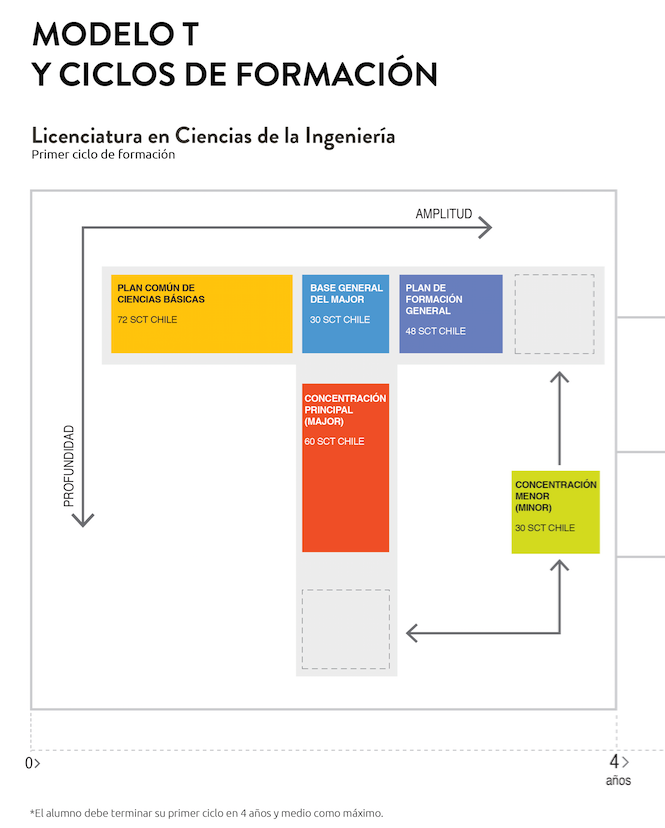
\includegraphics[width=0.5\textwidth]{./figures/model_t.png}
  \setcaptioncitation{\cite{student_manual}}
  \caption{Modelo T en el primer ciclo formativo}
  \label{fig:t_model}
	\end{center}
\end{figure}

De la figura \ref{fig:t_model} cabe destacar que el Minor complementa el aspecto profundidad o amplitud dependiendo del área del Major escogido.

Dado el objetivo de compatibilizar con mallas curriculares internacionales, los ciclos formativos miden su exigencia académica en créditos SCT-Chile, los cuales puede ser transformados a créditos UC gracias a la equivalencia entregada por la universidad. La distribución de carga académica por componente tanto en créditos SCT-Chile como créditos UC se distribuye en la siguiente tabla:

\begin{tabularx}{\linewidth}{@{}c c c@{}}
  \caption{Distribución de créditos SCT-Chile y UC en el primer ciclo formativo} \label{tab:distrution_credits}\\
  \toprule
  Componente & Créditos SCT-Chile & Créditos-UC
  \endhead
  \midrule
  Plan Común de Ciencias Básicas & 72 & 120\\
  \midrule
  Base General del Major & 48 & 80\\
  \midrule
  Plan de Formación General & 48 & 80\\
  \midrule
  Concentración Principal (Major) & 60 & 180\\
  \midrule
  Concentración Menor (Minor) & 30 & 50\\
  \bottomrule
\end{tabularx}

Esta estructura define la malla curricular del primer ciclo formativo, la cual puede ser visualizada en la ilustración \ref{fig:bachelor_study_plan}.

\begin{figure}
	\begin{center}
  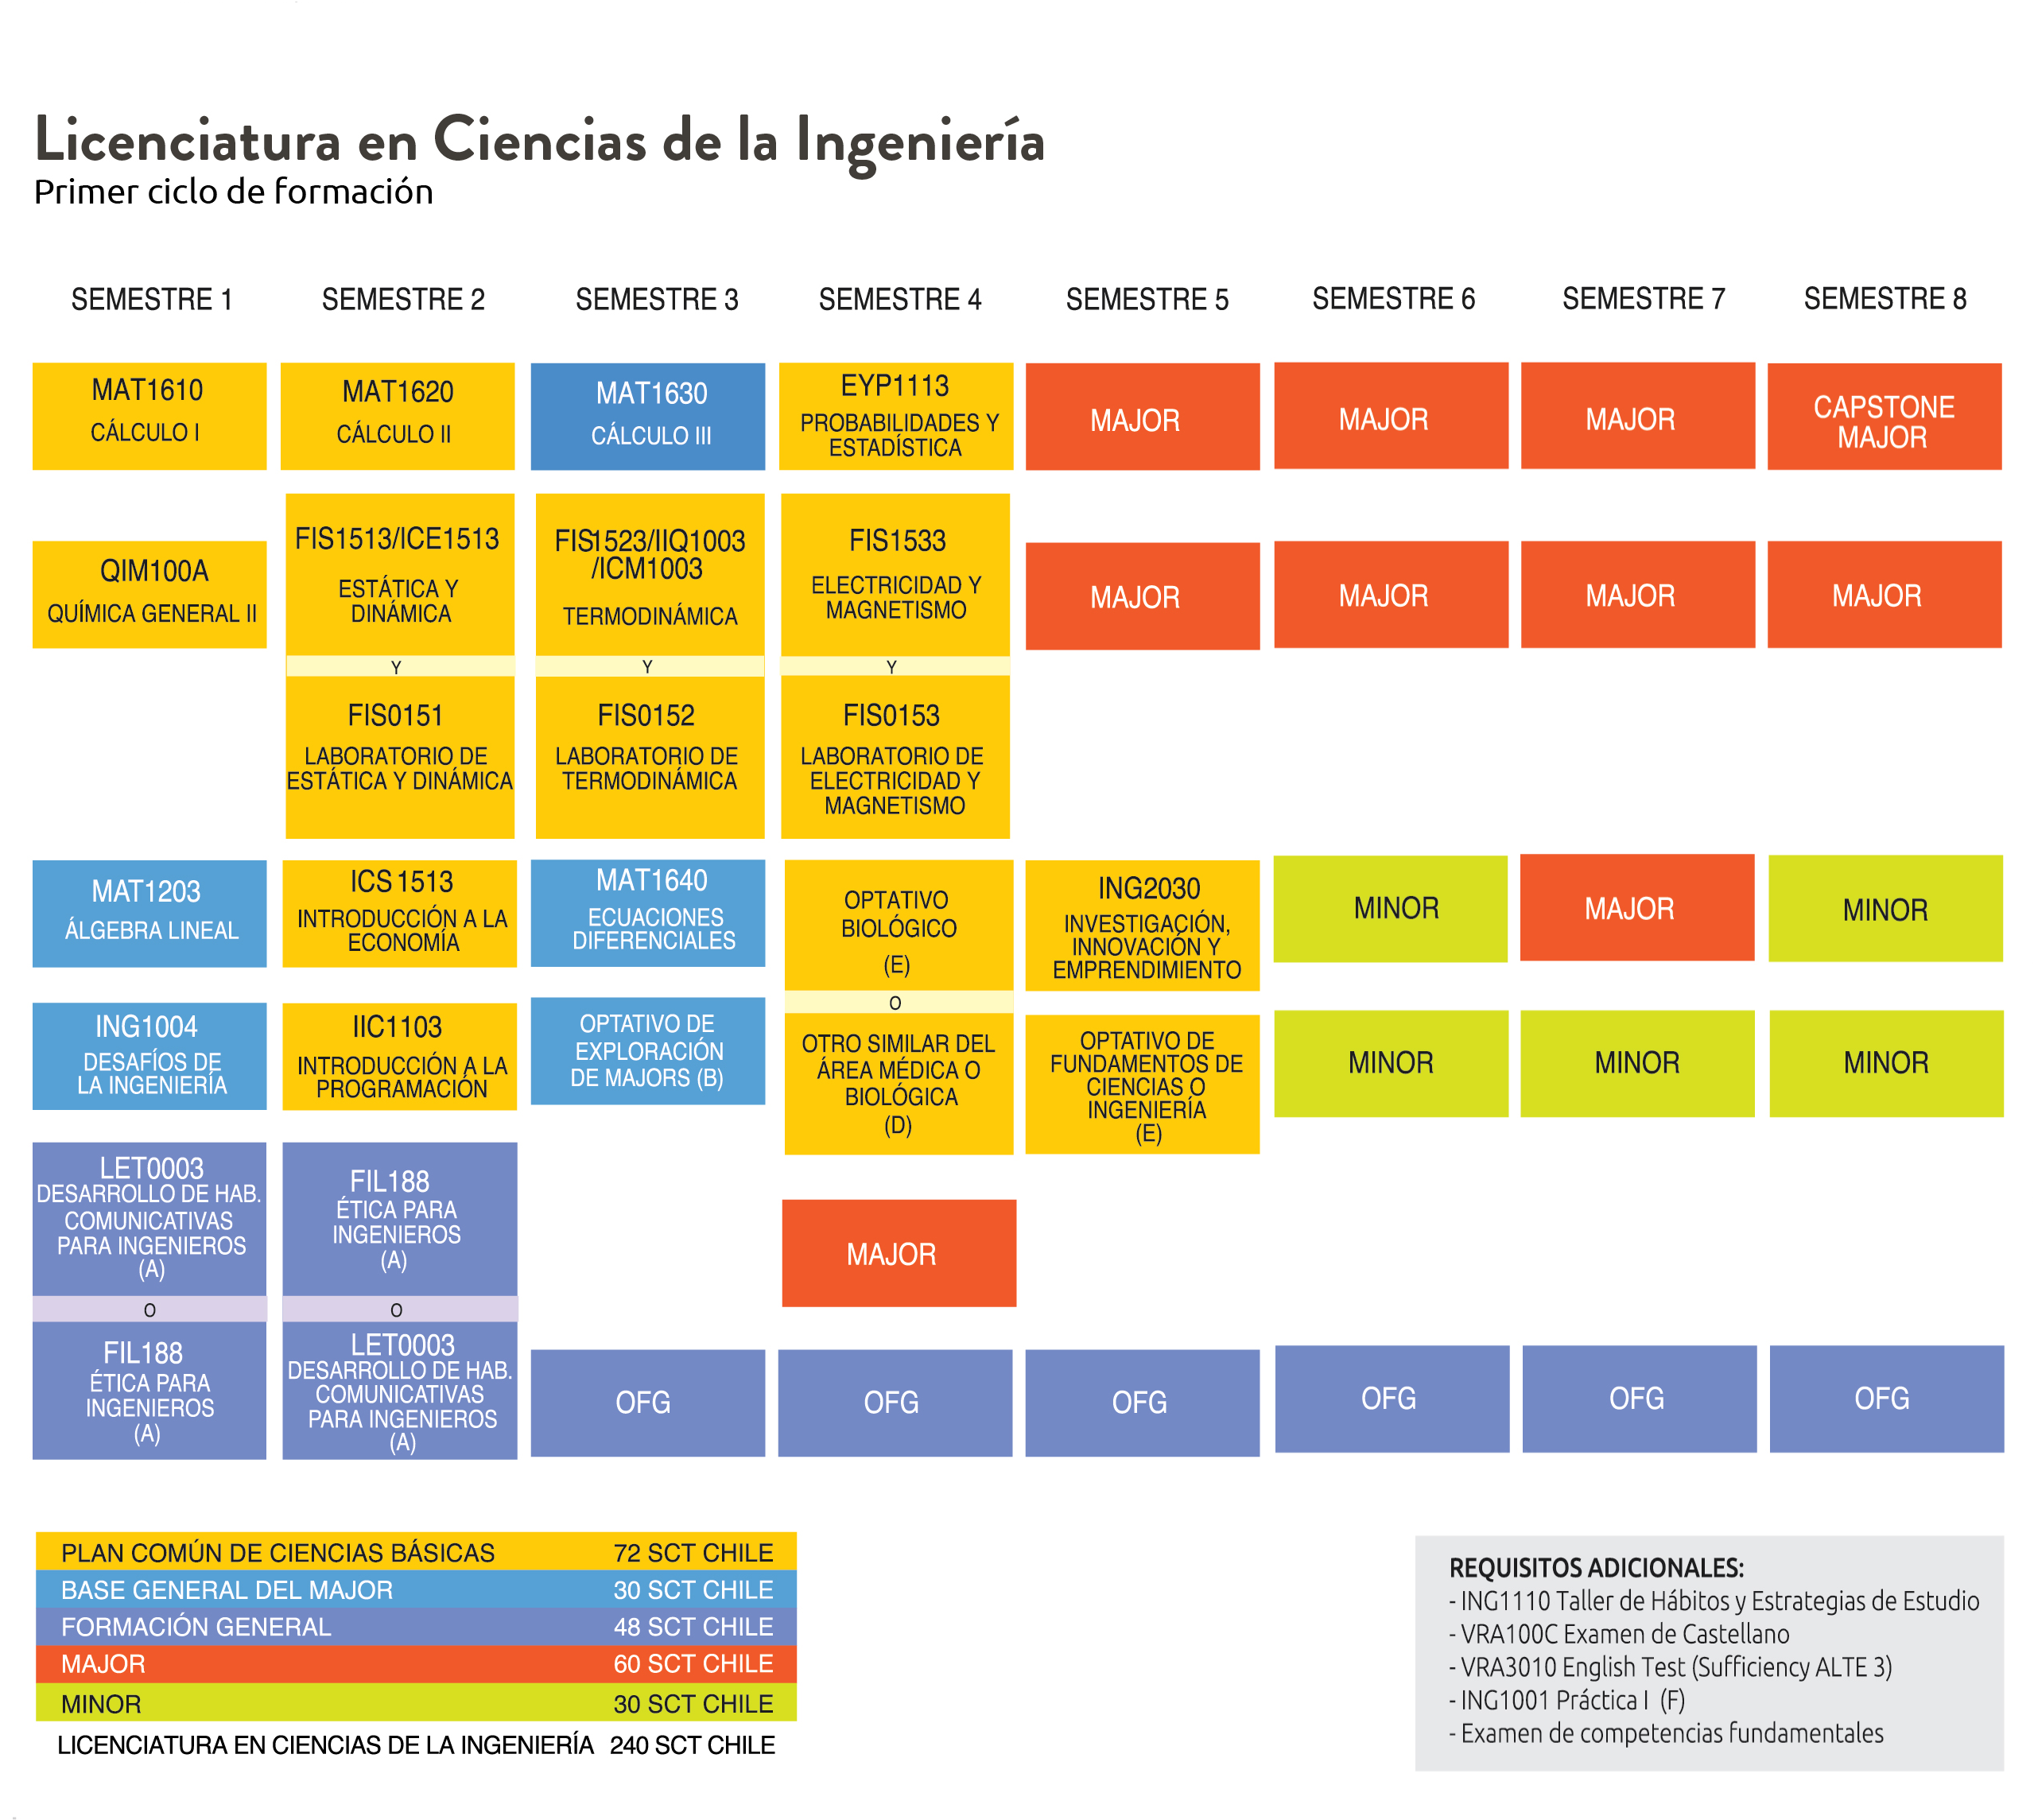
\includegraphics[width=0.7\textwidth]{./figures/malla_curricular.png}
  \setcaptioncitation{\cite{student_manual}}
  \caption{Malla curricular primer ciclo formativo}
  \label{fig:bachelor_study_plan}
	\end{center}
\end{figure}

La diversidad en la formación que puede escoger un alumno se encuentra en la conjunto Major-Minor que escoge, actualmente la Escuela de Ingeniería ofrece un total de 21 Majors, de los cuales 14 son disciplinarios y 7 interdisciplinarios, al mismo tiempo, entrega una oferta de 57 Minors entre los cuales, 32 son profundidad y 25 de amplitud. En el Anexo I se detalla los Majors y Minors disponibles.

Finalmente, con el objetivo de orientar a los alumnos hacia una elección de Major/Minor basada en sus intereses, se les solicita que hagan declaraciones de Major al término del segundo semestre y tercero para terminar con elección de Major y Minor al finalizar su cuarto semestre.

\subsubsection{Continuidad - Articulación Posterior a la Licenciatura \label{sec:degree_structure}}

El segundo ciclo formativo se inicia una vez obtenida la Licenciatura en Ciencias de la Ingeniería, el cual entrega los siguientes caminos a seguir:

\begin{enumerate}
  \item Continuidad a un título profesional de Ingeniería Civil UC.
  \item Continuidad a otros títulos profesionales UC. Hoy existen convenios para continuar estudios a los títulos de Médico Cirujano, Arquitecto y Diseñador UC.
  \item Articulación al título profesional Ingeniería UC y al Magíster en Ciencias de la Ingeniería o el Doctorado en Ciencias de la Ingeniería UC.
  \item Realizar un grado académico superior de postgrado (magister o doctorado) UC u otra.
  \item Salida al Mercado Laboral: Emprendimiento o Empleo Temprano.
\end{enumerate}

\section{Desafíos de información identificados \label{sec:challenges}}

El plan de estudios descrito recientemente fue implementado el año 2013, esto trae consigo una serie de cambios tanto en la comunidad de estudiantes por los nuevos conceptos establecidos como a nivel administrativo para la planificación de cursos para los diferentes ciclos y profesores para los cursos impartidos en cada uno. Esta situación se vuelve particularmente crítica en particular por varios cambios realizados en la planificación inicial de cada Major y/o Minor, así como también en las Articulaciones establecidas entre la Escuela de Ingeniería y otras unidades académicas como Diseño y Medicina. Tanto los cambios como la propia estructura flexible levantan un desafío a nivel de información en cómo realizar un seguimiento adecuado del plan de estudio que realiza cada alumno, para poder disponer de la mejor manera los recursos disponibles por la Escuela.

Las necesidades de información que se detectan para realizar un seguimiento adecuado del plan de estudios de cada alumnos pueden ser descritas en las siguientes categorías:

\begin{enumerate}
  \item Registro de cursos tomados por los alumnos en cada periodo académico.
  \item Registro de las declaraciones de Major realizadas por alumnos por periodo académico.
  \item Gestión de demanda de cursos para cursos, Major y Minor por parte de los alumnos de las diferentes generaciones del nuevo plan.
\end{enumerate}


\chapter[Capítulo 02 : Marco Teórico]{Capítulo 02 : Marco Teórico} \label{ch2}
\section{Introducción \label{sec:sec1}}
El presente trabajo se basa en conocimiento de Ingeniería de Software \textit{(Software Engineering)} y el proceso denominado Descubrimiento del Conocimiento \textit{(Knowledge Discovery)}. En el presente capítulo se exponen las definiciones de ambos campos, así como también los conceptos de cada área del conocimiento en Ciencias de la Computación.

\section{Ingeniería de Software \label{sec:software_engieering}}
De acuerdo a la \textit{Association for Computer Machinery} \cite{acm}, de ahora en adelante A.C.M., Ingeniería de Software o \textit{Software Engineering}, en adelante S.E., se preocupa de la construcción y mantención de software que posee las siguientes características:

\begin{enumerate}
  \item Comportamiento confiable y eficiente.
  \item Existe el modo de poder seguir desarrollando sobre ellos y al mismo tiempo mantenerlos.
  \item Satisfacen todos los requerimientos definidos por las necesidades de los clientes.
\end{enumerate}

Por su parte, \textit{Institute of Electrical and Electronics Engineers}, de ahora en adelante I.E.E.E. \cite{ieee} define S.E. como la aplicación de un enfoque sistemático, disciplinado y cuantificable para el desarrollo, operación y mantenimiento de software, es decir, la aplicación de ingeniería al software.

\subsection{Modelos y Ciclos de Vida del Desarrollo de Software \label{sec:software_engieering_models}}

A lo largo de la historia de S.E. se ha creado una diversidad de modelos o ciclos de vida para la creación y mantención de software. Cada modelo define la forma o estrategia en que las distintas actividades del proceso deben ser llevadas a cabo para el desarrollo y mantención del producto de software. A continuación se analizan los enfoques más descritos en la literatura actual.

\subsubsection{Modelo Cascada \label{sec:cascade_model}}

Este enfoque define una secuencia lineal de pasos para la creación de un software. Las etapas suelen incluir análisis de requisitos del sistema, análisis de requisitos de software, diseño preliminar, diseño, codificación, pruebas y mantenimiento. La siguiente ilustración muestra las etapas mencionadas anteriormente.

\begin{figure}[ht]
	\begin{center}
  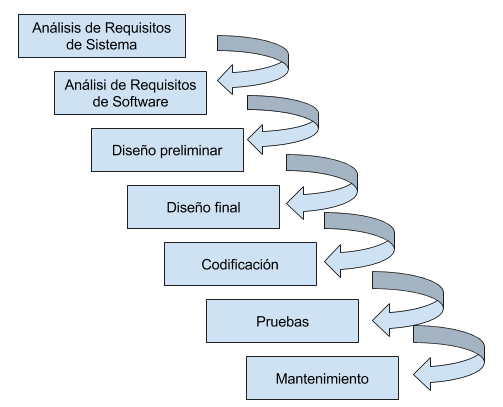
\includegraphics[width=0.5\textwidth]{./figures/chapter_02/01_cascade_phases.png}
  \setcaptioncitation{PENDIENTE}
  \caption{Fases del Modelo Cascada}
  \label{fig:cascade_model_phases}
	\end{center}
\end{figure}

El modelo de cascada se caracteriza por sus fases secuenciales, las cuales deben terminar de modo completo antes de iniciar una nueva. Adicionalmente, posee un fuerte enfoque en el levantamiento de requerimientos antes de iniciar cualquier actividad de código o de implementación del software, por lo cual se caracteriza por una intensa comunicación con los clientes o stakeholders en las fases iniciales, para luego dar protagonismo a las fases de codificación, pruebas y mantenimiento.

\textbf{Ventajas}
\begin{enumerate}
  \item Simple, permite una clara visualización de avance del proyecto.
  \item Se genera buena documentación que permite una clara planificación de los eventos dentro del proyecto.
  \item Etapa de codificación sólo se enfrenta después de tener un diseño robusto.
\end{enumerate}

\textbf{Desventajas}
\begin{enumerate}
  \item No es flexible frente a los cambios y deseos del cliente.
  \item Los errores sólo pueden ser detectados en etapas tardías de implementación.
  \item Cambios en los requerimientos agregan altísimos costos adicionales.
\end{enumerate}

\subsubsection{Modelo Incremental\label{sec:incremental_model}}

Este modelo consiste en una evolución del anterior mejorando la flexibilidad y al mismo tiempo disminuyendo  el tiempo de interacción con los stakeholders a lo largo de todo el proyecto. Con estos objetivos en mente, en vez de crear un proceso con etapas aisladas, se crea un proyecto que  puede ser diseñado, desarrollado e implementado en etapas sucesivas, incorporando al mismo tiempo la retroalimentación del cliente en etapas intermedias \cite{masssey}. El siguiente esquema ejemplifica la filosofía de este nuevo enfoque:

\begin{figure}[ht]
	\begin{center}
  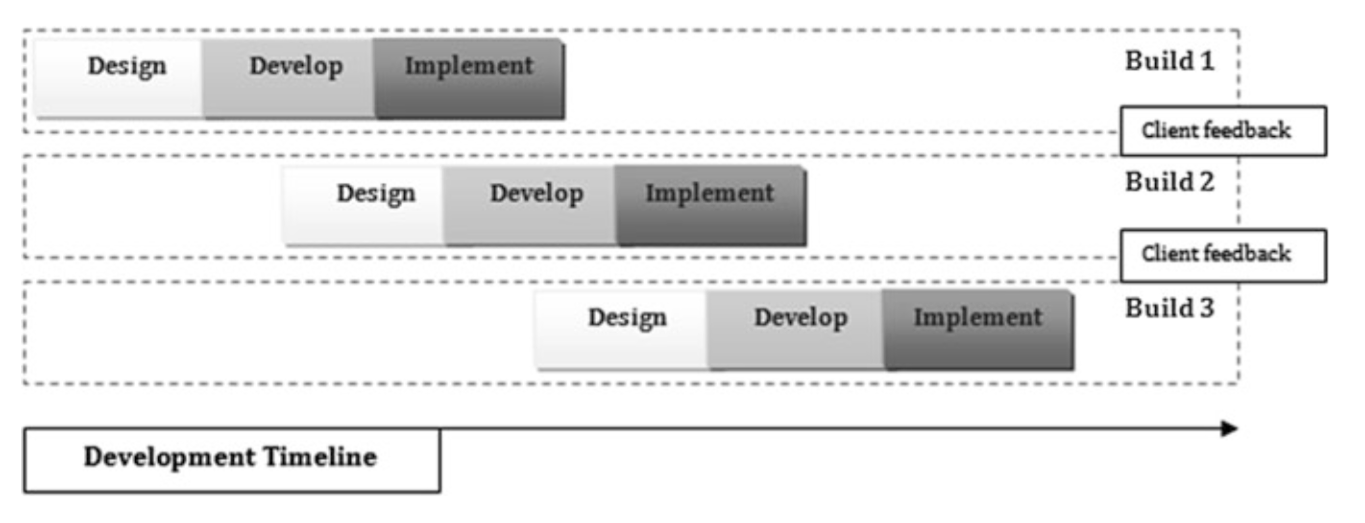
\includegraphics[width=\textwidth]{./figures/chapter_02/02_example_of_incremental_lyfe_cicle.png}
  \setcaptioncitation{PENDIENTE}
  \caption{Ejemplo de Ciclo de Vida del Modelo Incremental}
  \label{fig:cascade_incremental_model}
	\end{center}
\end{figure}

\textbf{Ventajas}
\begin{enumerate}
  \item Incorpora flexibilidad al permitir incorporar necesidades que no fueron previstas o consideradas en la etapa inicial del proyecto.
  \item Permite el desarrollo progresivo del proyecto hasta que está completo validando con los stakeholders durante todo el proyecto y no cuando éste haya finalizado.
\end{enumerate}

\textbf{Desventajas}
\begin{enumerate}
  \item La flexibilidad permitida por el proyecto puede hacer el proyecto más costoso debido a los constantes cambios que pueden realizarse.
  \item Al  incorporar nuevos elementos, debido a las etapas incrementales, puede tener problemas de incompatibilidad con versiones anteriores del software.
\end{enumerate}

\subsubsection{Rapid Application Development (RAD) \label{sec:incremental_model}}
Esta filosofía de desarrollo se basa en la idea de que los métodos desarrollados hasta los inicios de los 90 símplemente eran muy rígidos, en consecuencia no se podían aplicar de forma eficiente cuando las fechas de entrega cobran importancia. La ideología se basa en la  entrega rápida de software mientras se mantiene una alta calidad en la implementación desarrollada. Esta metodología fue desarrollada y formalizada por James Martin en el mismo horizonte de tiempo.

Este proceso de creación posee dos modalidades, la primera consiste en 4 fases secuenciales de tiempo : planificación de requerimientos, diseño desde el punto de vista del usuario, construcción y transición a la siguiente fase. En la segunda modalidad se fusionan las fases de planificación de requerimientos y diseño en una sola de análisis. Todas las fases de desarrollo en ambas modalidades se desarrolla en un espacio de tiempo determinado denominado timebox, donde se priorizan las actividades en función de las necesidades del negocio sin importar el desafío técnico al cual se ven enfrentadas \cite{gottesdiener}. A continuación se presenta un posible esquema de trabajo bajo esta metodología:

\begin{figure}[ht]
	\begin{center}
  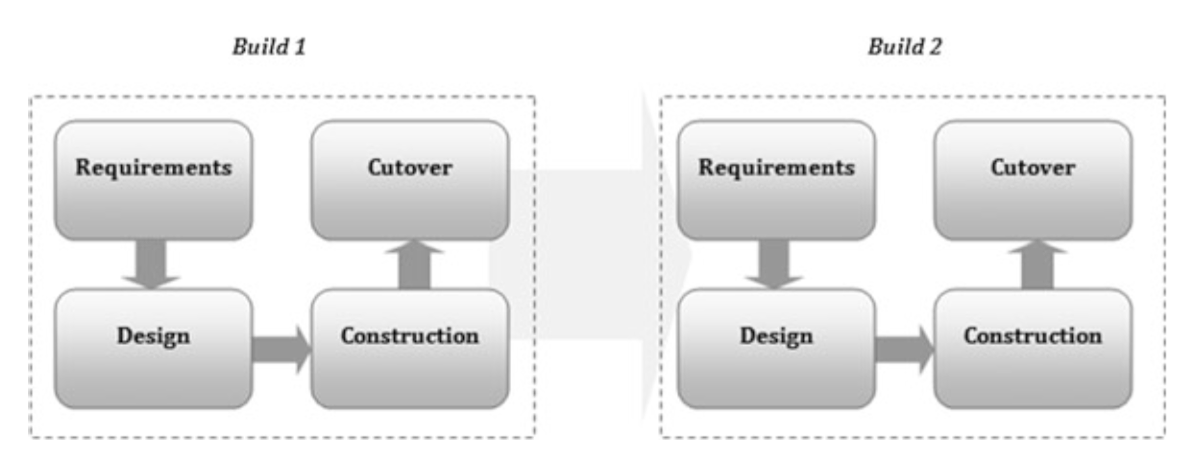
\includegraphics[width=\textwidth]{./figures/chapter_02/03_succession_of_increments.png}
  \setcaptioncitation{PENDIENTE}
  \caption{Sucesión de Incrementos en Timebox de 4 (o 3) pasos}
  \label{fig:succession_of_increments}
	\end{center}
\end{figure}

\textbf{Ventajas}
\begin{enumerate}
  \item Al enfocarse en prioridades de negocio sin importar dificultades técnicas permite entregar una implementación que satisface las necesidades más críticas de los \textit{stakeholders}.
  \item Al tener un tiempo específico de desarrollo se mantiene un paso a producción marcado por hitos.
  \item Debido a que los espacios de tiempo de desarrollo entre bloques no son necesariamente del mismo horizonte temporal es posible adaptarlos a las nuevas necesidades que vayan surgiendo en el transcurso del proyecto.
  \item Posee una comunicación constante para el desarrollo de cada fase.
\end{enumerate}

\textbf{Desventajas}
\begin{enumerate}
  \item Sólo puede ser usada cuando las personas que lo desarrollan tienen un alto nivel técnico y una gran capacidad de trabajo en equipo, debido a que los tiempos de desarrollo necesitan ser lo más preciso posible por cada bloque.
  \item Es posible que se creen expectativas falsas por parte de las personas que gestionan el proyecto al ser trabajado bajo espacios específicos de tiempo, lo que podría generar discusiones internas con el equipo de desarrollo.
\end{enumerate}

\subsubsection{Enfoque Ágil \label{sec:incremental_model}}

Esta modalidad de desarrollo nace específicamente en el año 2001 con la publicación del Manifiesto Ágil, en donde se da a conocer un \textit{framework} de cómo construir un software en un ambiente de constantes cambios y al mismo tiempo mantener un alto nivel de calidad de implementación y satisfacción al cliente. Existen 12 principios declarados en este manifiesto, los cuales pueden ser resumidos en las siguientes declaraciones \cite{agile}:

\begin{enumerate}
  \item La satisfacción del cliente es la principal prioridad.
  \item Cambios en los requerimientos son bienvenidos, no son más un obstáculo.
  \item El \textit{software} es entregado regularmente en constantes \textit{release}.
  \item Los responsables de negocio y los desarrolladores trabajamos juntos de forma cotidiana durante todo el proyecto.
  \item Individuos motivados son una pieza vital para el éxito del proyecto.
  \item Conversaciones cara a cara es esencial para una exitosa colaboración.
  \item El \textit{software} funcionando es la medida principal de progreso.
  \item El desarrollo sostenible debe ser alentado.
  \item Enfocado en bases técnicas y diseño de calidad.
  \item Simplicidad debe ser favorecida.
  \item La mejor forma de gestionar un proyecto es con equipos auto organizados.
  \item Debe haber constantes discusiones para el mejoramiento del equipo.
\end{enumerate}

En términos generales es posible establecer 4 etapas para el desarrollo bajo este enfoque  \cite{agile}:

\begin{description}
  \item[1. Selección y aprobación del proyecto] Los stakeholders (administradores, desarrolladores, clientes, entre otros) definen de modo conjunto el alcance, propósito y requerimientos del producto o implementación.
  \item[2. Iniciación del proyecto] El equipo de trabajo es construido en base a los requerimientos anteriormente establecidos. Adicionalmente, se establece la infraestructura de trabajo y se procede a la instalación de las herramientas tecnológicas a ocupar. En general, se establecen espacios de tiempo de trabajo para el equipo y reuniones de acuerdo a las necesidades del proyecto.
  \item[3. Construcción basada en iteraciones] Las iteraciones consisten en dos etapas, planificación y construcción. La idea es que al final de cada iteración se obtenga una pieza de software terminada.
  \item[4. Entrega de producto maduro \textit{(product release)}] Esta fase final está caracterizada nuevamente por dos etapas, pruebas y mejoramiento así como también de la documentación necesaria para el entendimiento del proyecto.
\end{description}

El esquema \ref{fig:agile_development_life_cycle} muestra el proceso genérico bajo cualquier proceso con enfoque ágil:

\begin{figure}[ht]
	\begin{center}
  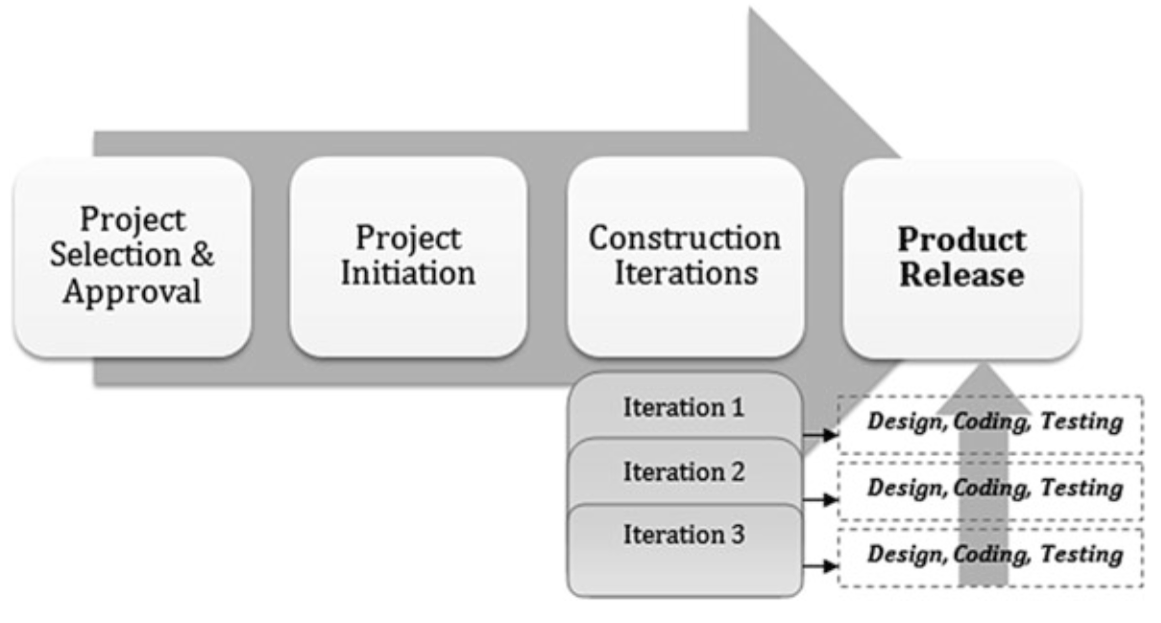
\includegraphics[width=0.85\textwidth]{./figures/chapter_02/04_agile_development_life_cycle.png}
  \setcaptioncitation{PENDIENTE}
  \caption{ Ejemplo del Ciclo de Vida del Desarrollo Ágil}
  \label{fig:agile_development_life_cycle}
	\end{center}
\end{figure}

\subsection{Metodologías de Desarrollo de Software \label{sec:methodologies}}

Un modelo o ciclo de vida puede ser considerado como una estructura de referencia, una estrategia general para enfrentar el desarrollo, pero no prescribe el modo concreto de llevarlo a cabo. La forma específica de cómo llevar a cabo el proyecto la define una metodología orientada por un determinado modelo o enfoque.

Dentro de los modelos mencionados anteriormente él más relevante hoy en día es enfoque ágil debido a los cambios que ha sufrido la industria tanto a nivel tecnológico como social. Desde su nacimiento en el año 2001 por la declaración del Manifiesto Ágil han surgidos diversas metodologías, las cuales enfrentan diferentes desafíos impuestos por los supuestos de esta modalidad de desarrollo, tales como incorporación de cambios en cualquier momento del proyecto. A continuación se describen dos de las metodologías más populares que permiten implementar el enfoque ágil, éstas son Scrum y Extreme programming (XP). La figura \ref{fig:agile_methodologies_used} muestra la dominancia de Scrum entre las metodologías ágiles:

\begin{figure}[ht]
	\begin{center}
  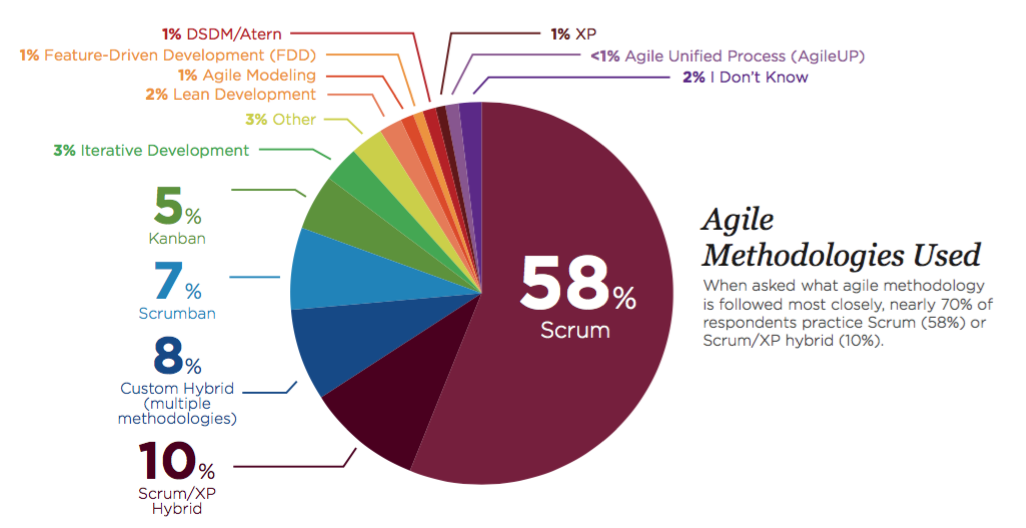
\includegraphics[width=0.85\textwidth]{./figures/chapter_02/05_agile_methodologies_used.png}
  \setcaptioncitation{PENDIENTE}
  \caption{Uso de Metodologías Ágiles}
  \label{fig:agile_methodologies_used}
	\end{center}
\end{figure}

Como se aprecia sólo Scrum cubre más del $50\%$ de la industria. Si bien XP representa sólo un $1\%$, es la base de Scrum/XP Hybrid que es usado por $10\%$ de la industria y es muy usada en grupos pequeños de desarrollo. Por lo tanto, en el desarrollo de este trabajo se consideraron tanto Scrum como XP.

\subsubsection{Scrum \label{sec:scrum}}

Esta metodología se basa principalmente en cómo un equipo debe funcionar y las relaciones que los miembros de éste establecen. Para lograr este objetivo se definen roles, eventos, artefactos y reglas. Cada componente dentro de este marco de referencia sirve para un propósito específico que son esenciales para éxito de su aplicación \cite{scrum_guide}. A continuación se ilustra la forma de trabajo en esta metodología en dos aspectos, primero la figura \ref{fig:scrum} se identificación los elementos presente en la metodología y a continuación en la figura \ref{fig:scrum_framework} se muestra cómo estos interactúan en el transcurso de un proyecto.

\begin{figure}[ht]
	\begin{center}
  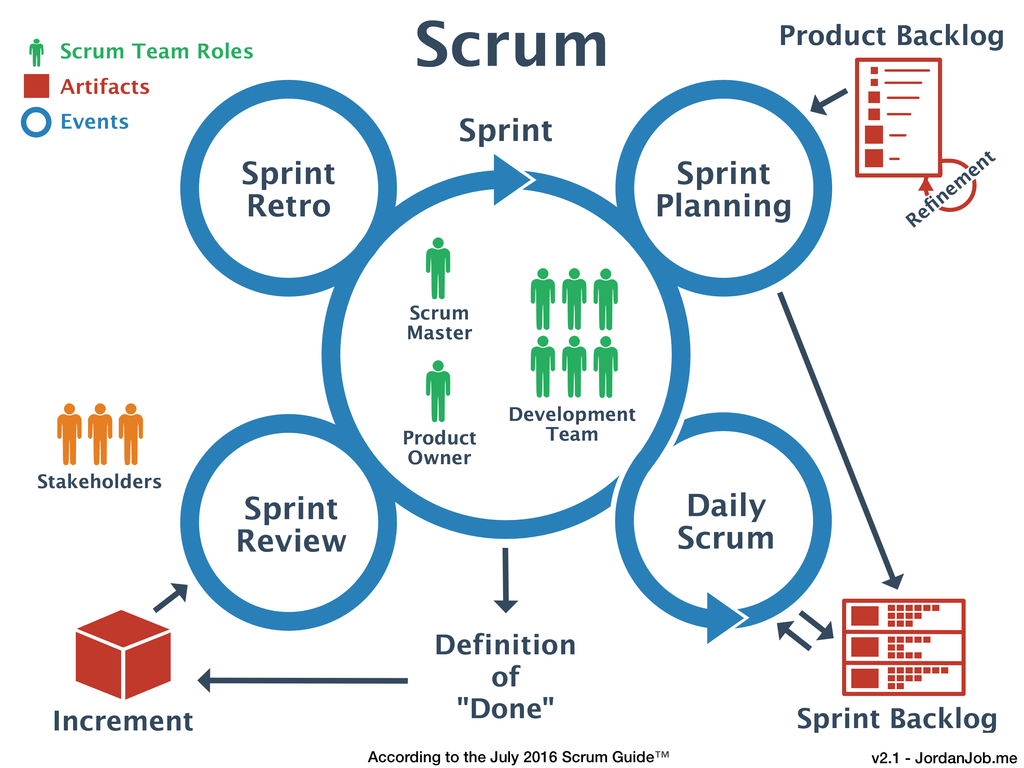
\includegraphics[width=0.85\textwidth]{./figures/chapter_02/06_scrum.png}
  \setcaptioncitation{PENDIENTE}
  \caption{Elementos presenten en Scrum}
  \label{fig:scrum}
	\end{center}
\end{figure}

\begin{figure}[ht]
	\begin{center}
  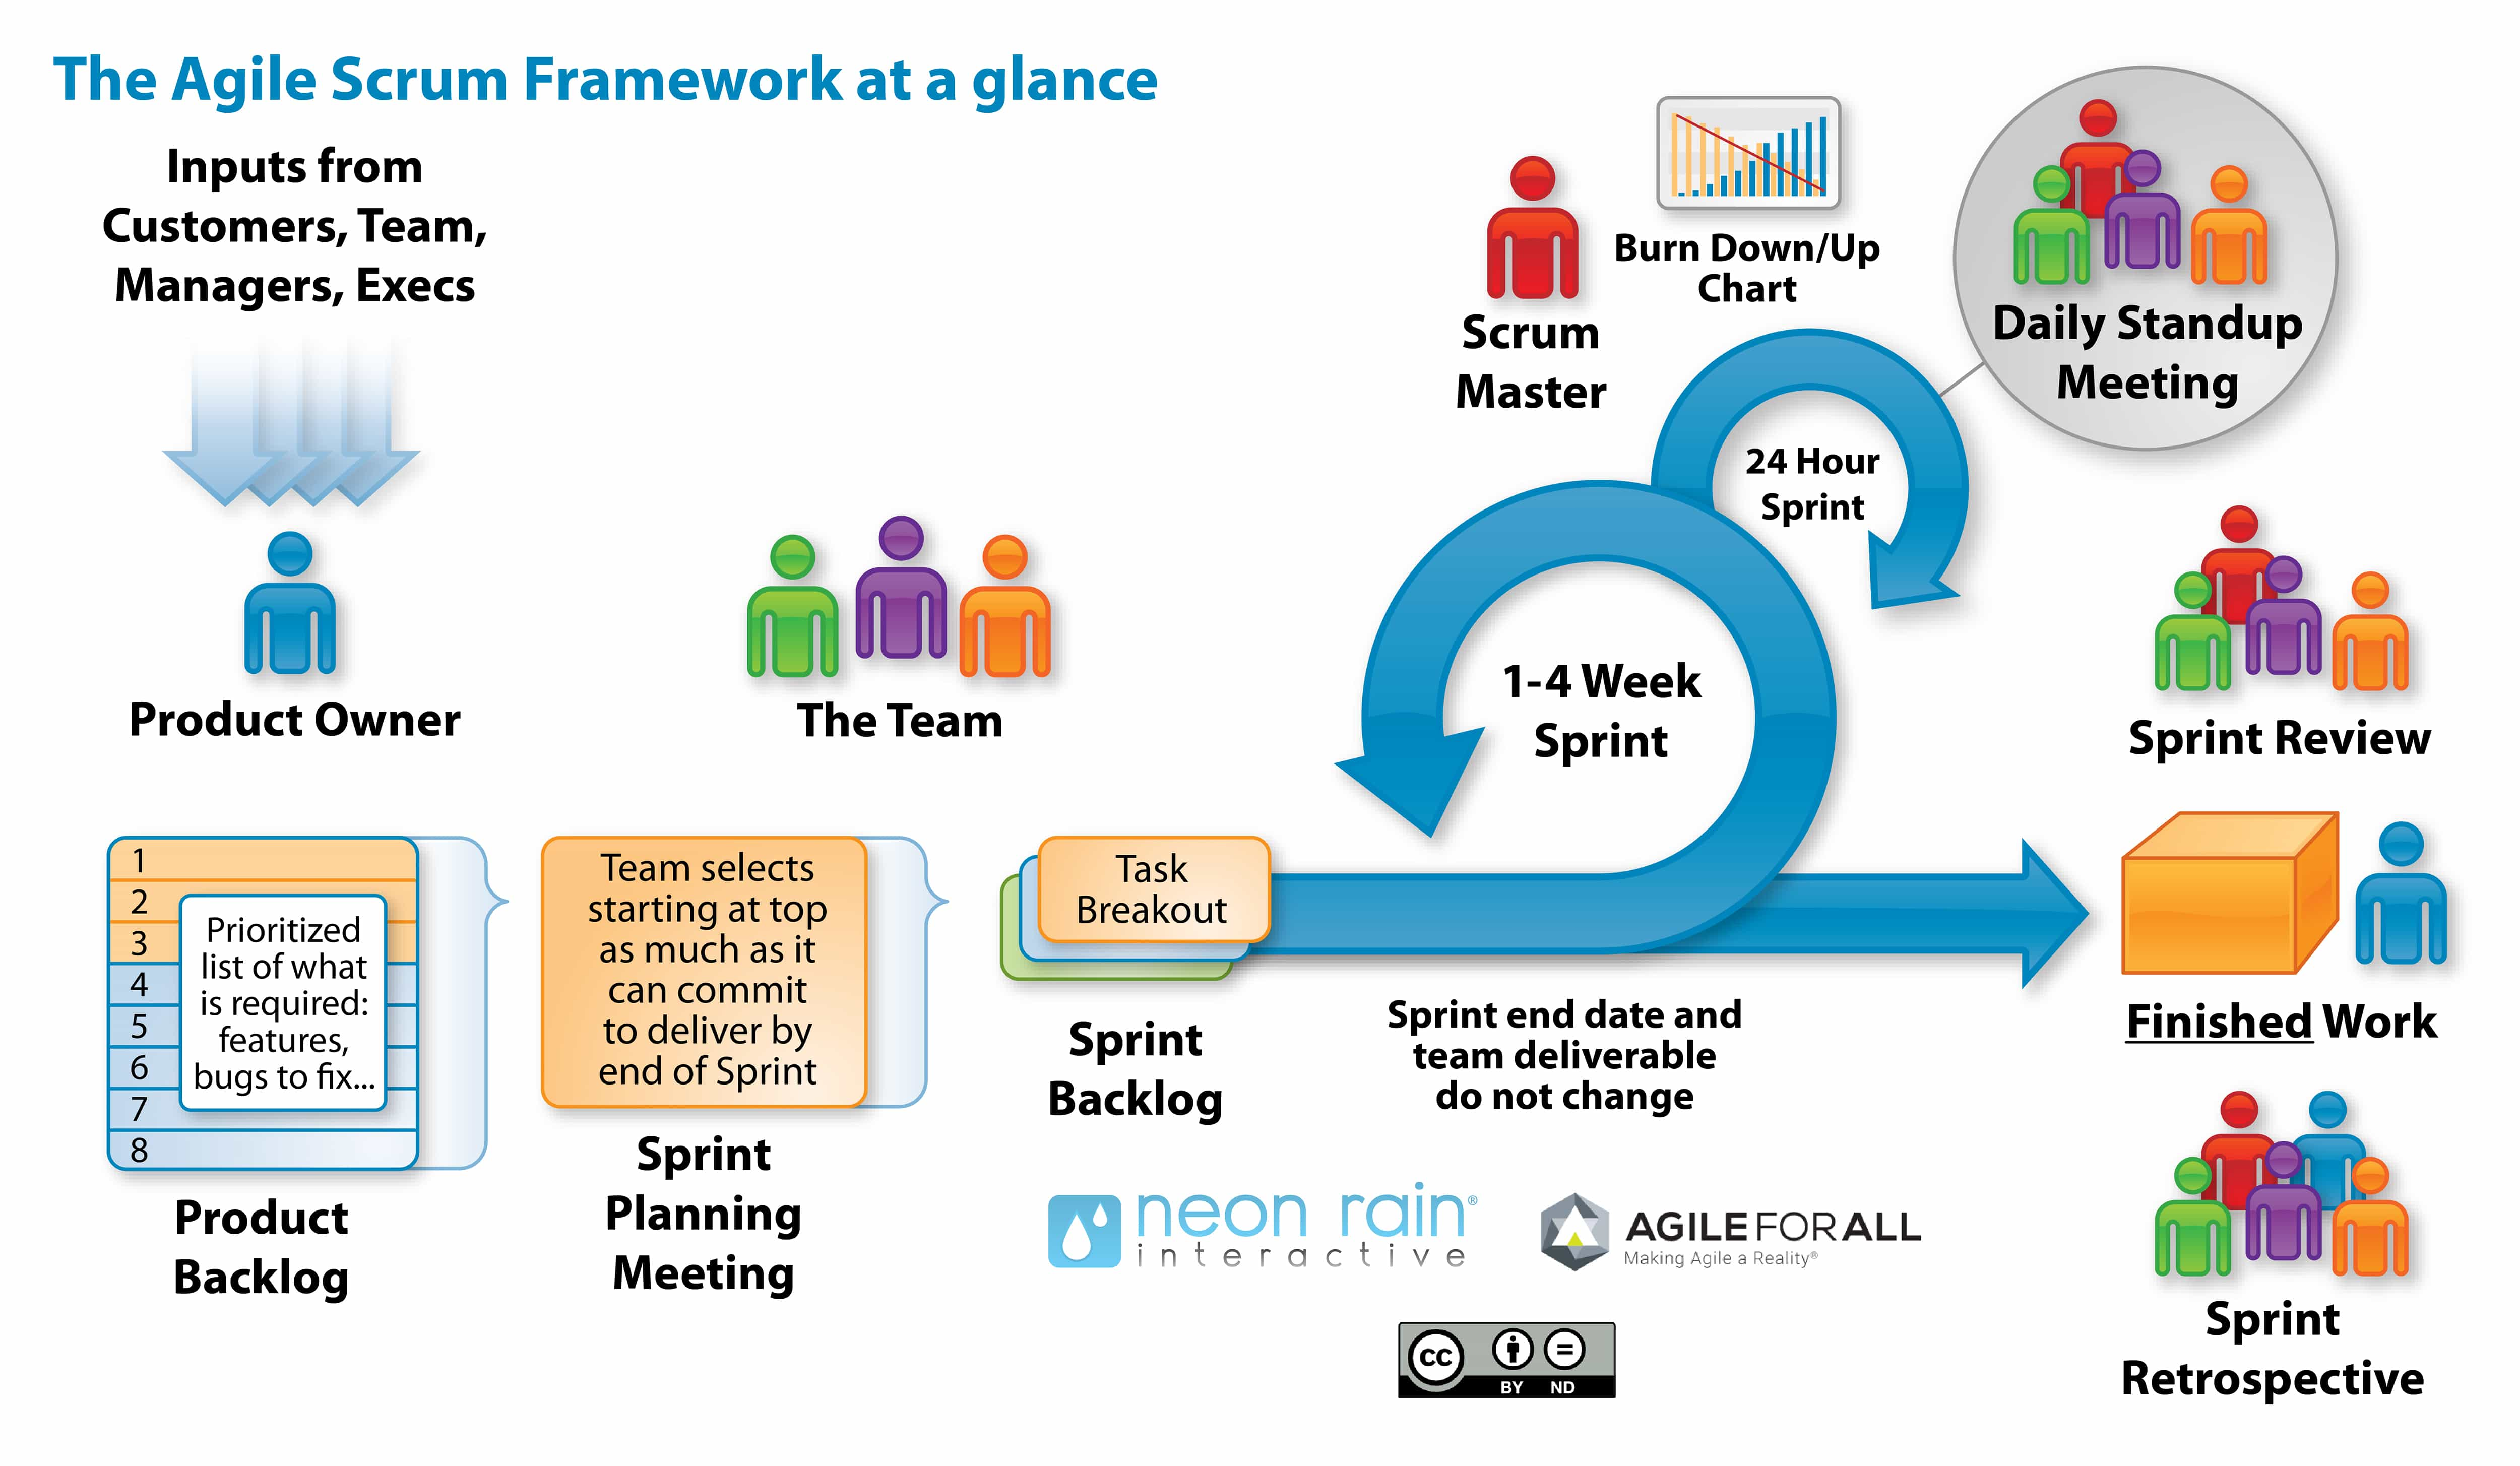
\includegraphics[width=1\textwidth]{./figures/chapter_02/07_scrum_framework.jpg}
  \setcaptioncitation{PENDIENTE}
  \caption{Scrum Framework}
  \label{fig:scrum_framework}
	\end{center}
\end{figure}

Los roles identificados en este metodología son:

\begin{description}[leftmargin=10em,style=nextline]
  \item[1. \textit{Stakeholder}] Corresponde a todas aquellas personas que se involucran en el proyecto, desde los usuarios finales hasta quienes financian el desarrollo del proyecto. Se identifica a todos aquellos que poseen algún interés una vez que el proyecto esté finalizado.
  \item[2. \textit{Product Owner}] Es el encargo de entender el contexto en el cual se desenvuelve el proyecto y en base a eso llevar a cabo el levantamiento de requerimientos del proyecto.
  \item[3. \textit{Scrum Master}] Es el responsable de verificar que la metodología Scrum sea aplicada de forma correcta, así como también el encargado de proporcionar a cada miembro del equipo los elementos que necesite para llevar a cabo su tarea. Este rol debe estar al servicio tanto del \textit{Product Owner} como para los miembros del equipo de desarrollo.
  \item[4. \textit{Development Team}] Son los responsables de la creación del proyecto en base a los requerimientos entregados por el \textit{Product Owner}.
\end{description}

Por su parte, la definición de los artefactos en esta metodología son:

\begin{description}[leftmargin=10em,style=nextline]
  \item[1. \textit{Product Backlog}] Es una lista ordenada de todas las necesidades del producto/proyecto y es la única fuente de requerimientos existente. El responsable de su escritura es el Product Owner, quien debe procurar por su contenido, disponibilidad y orden. Se debe indicar que nunca está completo y permanece en frecuente cambio frente a los diferentes requerimientos que el proyecto pueda ir necesitando. A modo general este artefacto posee las funcionalidades, requerimientos, mejoras y reparaciones para las próximas versiones del producto. Los elementos presentes poseen nombre o título, atributos que permiten describirlo, orden, estimación y valor para el proyecto \cite{scrum_guide}.
  \item[2. \textit{Sprint Backlog}] Es el conjunto de ítems seleccionados del Product Backlog que conforman el siguiente entregable del producto/proyecto que se está desarrollando. Se puede interpretar como la proyección de lo que será el software en su siguiente fase, donde todos los elementos presentes en este conjunto se considerarán terminados.
  \item[3. \textit{Increment}] Es la suma de todos los elementos desarrollados en un Sprint Backlog. Este debe considerarse terminado y listo para ser usado en la próxima versión del software.
\end{description}

Finalmente, se definen eventos dentro de Scrum con el objetivo de mantener una comunicación regular y eliminar la necesidad de encuentros. Cada evento posee una duración limitada y que puede varias según el proyecto así como también del equipo quien implemente la metodología, sin embargo, existen un periodo de tiempo recomendado en cada caso.

Los eventos presentes en Scrum son \cite{scrum_guide}:

\begin{description}[leftmargin=10em,style=nextline]
  \item[1. \textit{Sprint}] Se considera como el corazón de Scrum debido a que es el periodo de tiempo base en el cual se entrega un increment (incremento) del software. La duración recomendada para un sprint es un mes o semanas y es ideal que mantenga la misma duración durante todo el proyecto. Dentro de este periodo de tiempo ocurre el sprint planning, daily scrum, sprint review y, finalmente, sprint retrospective.
  \item[2. \textit{Sprint Planning}] Periodo de tiempo en el cual se planifica el trabajo y orden del mismo a realizarse en durante el sprint. El tiempo máximo para un sprint planning es de 8 horas cuando el tiempo del sprint es de un mes. El scrum master es el responsable de la gestión y la ejecución de esta fase. Por otro lado, se entiende que este periodo tiene por objetivo responder ¿qué elementos formarán parte del próximo increment ? y ,al mismo tiempo, ¿qué trabajo se realizará para cumplir el requerimiento descrito en el Product Backlog?

  \item[3. \textit{Dialy Scrum}] Consiste en una reunión de 15 minutos de duración donde el equipo de desarrollo sincroniza y crea el plan de desarrollo para las próximas 24 horas. Este trabajo se hace en base a la última reunión realizada. Adicionalmente, los miembros del equipo explican qué hicieron en el último daily scrum, que harán en el actual y de forma conjunta identifican e informan los problemas que han ocurrido y los que podrían ocurrir para el desarrollo del siguiente daily scrum.

  \item[4. \textit{Sprint Review}] Es una reunión informal con máxima duración de 4 horas donde los miembros del equipo de desarrollo identifican los logros obtenidos al final del sprint. Es una instancia en donde es posible modificar el Product Backlog. En esta reunión deben participan  stakeholders invitados por el Product Owner y todos los miembros de la metodología. Los principales objetivos de este intervalo de tiempo son:
    \begin{enumerate}
      \item Qué se hizo y qué no hizo.
      \item Se explican en detalle los problemas ocurridos y cómo fueron resueltos.
      \item Se discute de modo general qué elementos son importantes en base al avance logrado para el siguiente sprint planning.
      \item Se discute el estado del Product Backlog y se modifica en base al incremento logrado, a los cambios provenientes de los stakeholders así como también de los eventos externos del proyecto.
    \end{enumerate}

  \item[5. \textit{Sprint Retrospective}] Es un encuentro donde el equipo de desarrollo analiza su modo de trabajo y crea un plan de mejoras para ser atacadas en el próximo sprint. Se inspeccionan todos los ámbitos dentro de un equipo los miembros involucrados en el proyecto, relaciones entre ellos, procesos y herramientas utilizadas. Esta reunión se recomienda una duración máxima de 3 horas y se realiza al finalizar el sprint.
\end{description}

\subsubsection{Extreme Programming \label{sec:extreme_programming}}
Esta metodología basa su funcionamiento en 2 principios principales: simplicidad y eficiencia. Con el objetivo de lograr estos principios se definen los siguientes 4 valores o elementos, los cuales poseen sus propias características:

\begin{enumerate}
  \item \textbf{Comunicación (Communication)}\mbox{}\\ Enfocada en lograr la cooperación y buena relación entre los miembros del equipo, para lograr esto se propicia la participación constante del cliente, programación a pares y poseer dentro del equipo de desarrollo una estandarización de código.

  \item \textbf{Diseñar de modo simple (Simplicity)} \mbox{}\\ Orienta a que los elementos que se crean sean simples y basado en el pensamiento asociativo usando el mundo real como referencia, es decir, el uso de metáforas. Esto incluye las mejoras que se realizan a través de \textit{refactoring} \dictionary{refactoring}.

  \item \textbf{Retroalimentación constante (Feedback)} \mbox{}\\ Consiste en definir los modos para asegurarse que el software es aceptado tanto por el equipo de desarrollo como los clientes. Para ello necesita de testing continuo, integración continua (recomendado al menos una vez al día) y ,finalmente, basar las entregas en pequeñas funcionalidades.

  \item \textbf{Aceptación de nuevos cambios (Courage)} \mbox{}\\ Consta de todas las acciones usadas para la organización del proyecto y del equipo, para ello motiva realizar el levantamiento de requerimientos en base a relatos de usuario para el proyecto y a nivel de equipo estimula el concepto de propiedad de código colectiva.
\end{enumerate}

Los tiempos de desarrollo en XP se basan en iteraciones de 3 semanas en las cuales se recomienda seguir las siguientes 12 prácticas de software:

\begin{enumerate}
  \item Planificación del proceso : En esta instancia es donde se recomienda usar relatos de usuarios para la descripción de las funcionalidades del software.
  \item Entregables pequeños.
  \item Entregables pequeños.
  \item \textit{Test Driven Develpment} \dictionary{tdd}.
  \item \textit{Refactoring} \dictionary{refactoring}.
  \item Mantener el diseño simple.
  \item Programación a Parea \dictionary{pair_programming}.
  \item Propiedad colectiva del código.
  \item Uso de estándares de programación.
  \item Integración continua \dictionary{continuous_integration}.
  \item Mantener al cliente cercano.
  \item Mantener un buen clima laboral.
  \item Utilización de metáforas para el diseño : Consiste en crear un lenguaje común para el equipo de desarrollo y clientes con el objetivo de que todos puedan comprender los conceptos y definiciones usadas en el proyecto del mismo modo.
\end{enumerate}

La metodología es poco prescriptiva (en comparación a Scrum) pero existen prácticas sugeridas para organizar el flujo de trabajo. Por ejemplo, el sitio ExtremProgramming.Org sugiere el esquema presentado en la figura \ref{fig:extreme_programming_workflow}.

\begin{figure}[ht]
	\begin{center}
  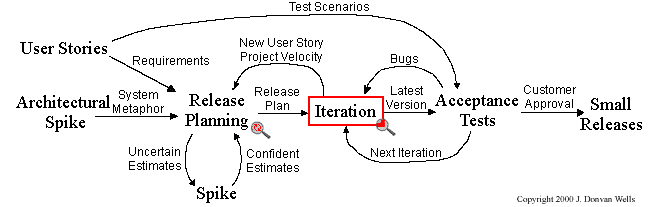
\includegraphics[width=1\textwidth]{./figures/chapter_02/08_extreme_programming_project.png}
  \setcaptioncitation{PENDIENTE}
  \caption{Flujo de Trabajo en \textit{Extreme Programming}}
  \label{fig:extreme_programming_workflow}
	\end{center}
\end{figure}

\subsection{Levantamiento de Requerimientos \label{sec:requirements}}

De acuerdo al Glosario Estándar de Ingeniería de Software de la IEEE \cite{ieee_glosary}, el concepto de requisito puede entenderse de acuerdo a alguna de las siguientes definiciones:

\begin{enumerate}
  \item Condición o capacidad necesaria por un usuario para solucionar un problema o alcanzar un objetivo.
  \item Condición o capacidad que debe ser encontrada o poseer un sistema o algún componente de éste que satisfaga un contrato, un estándar, especificación u otra formalidad impuesta por documentación.
\end{enumerate}

Al mismo tiempo, de acuerdo a la guía PMBOK \cite{pmbok_guide}, identifica 3 categorías:

\begin{enumerate}
  \item \textbf{Requerimientos del Negocio}\mbox{}\\ Describen las necesidades de alto nivel de la organización como un todo, tales como, oportunidades o problemas del negocio, y los motivos por los cuales un proyecto ha sido iniciado.
  \item \textbf{Requerimientos de los \textit{Stakeholders}}\mbox{}\\ Describen las necesidades de uno o varios \textit{stakeholders}.
  \item \textbf{Requerimientos de la Solución} \mbox{} \\ Describen las funcionalidades, funciones o características de un producto, servicio o resultado que resuelve los requerimientos del negocio y de los stakeholder. Dentro de los requerimientos de solución es posible encontrar dos tipos:
    \begin{enumerate}
      \item \textbf{Requerimientos funcionales:} Describen el comportamiento del producto o desarrollo. Por ejemplo: procesos, información, base de datos e interacciones del usuario y producto.
      \item \textbf{Requerimientos no funcionales:} Entrega los criterios medibles a través de los cuales un sistema puede comprobar su funcionamiento. Las principales áreas en las cuales se definen estos criterios son rendimiento, nivel de seguridad, escalabilidad, entre otros.
    \end{enumerate}
\end{enumerate}

Por lo descrito anteriormente, las metodologías permiten la captura de requisitos de diferentes maneras, las más usuales para los requerimientos del negocio y \textit{stakeholders} corresponden a \textit{focus groups} \dictionary{focus_group}, reuniones y encuestas. De modo transversal a las metodologías, este procedimiento de entendimiento donde se desarrolla el producto o \textit{software} finaliza con un objetivo principal y una serie de objetivos secundarios que deben cumplirse al término de éste. Esta dinámica en las metodologías mencionadas anteriormente se realiza en una etapa específica o designa un responsable para ello, por ejemplo, en Scrum el responsable de este procedimiento durante todo el proyecto es el \textit{Product Owner}. Adicional a esto, al momento de especificar los requerimientos de solución, debido a que los requisitos funcionales describen comportamiento, el cual dentro de lo posible debe ser interpretado del mismo por todo los miembros del equipo, presentan la necesidad de realizarse bajo una estructura o esquema de descripción específico. Esta situación no sucede con los requerimientos no funcionales, debido a que ellos presentan métricas  y sus criterios para ser evaluadas , por ejemplo, el tiempo de carga al sitio inicial del \textit{software} no debe ser mayor a 1 segundo.

Dentro de las técnicas de descripción o \textbf{levantamiento de requisitos funcionales}, se encuentran Casos de Usos \textit{(Use Cases)} y Relatos de Usuarios \textit{(User Stories)}.

\subsubsection{Casos de Uso \label{sec:use_cases}}

De Acuerdo a Cockburn \cite{uses_cases_writing}, un caso de uso se define como la descripción del comportamiento del sistema bajo varias condiciones que responden a la necesidad de uno o varios \textit{stakeholders}. Adicionalmente, se espera que un caso de uso sea fácil de leer, para una completa identificación de las necesidades se propone las siguientes partes para una descripción completa:

\begin{enumerate}
  \item \textbf{Nombre \textit{(Name)}}\mbox{}\\ Correspondiente al nombre de la acción que se desea realizar.
  \item \textbf{Objetivo en Contexto \textit{(Goal in Context)}}\mbox{}\\ Menciona las motivaciones del actor principal para la realización de sus acciones, así como también la descripción del entorno en el cual las realiza.
  \item \textbf{Alcance del diseño \textit{(Design Scope)}} \mbox{} \\ Corresponde a la definición de que se desarrolla y no desarrolla dentro del proyecto. Con el objetivo de describir el alcance dentro de un contexto Cockburn define los siguientes niveles o tipos de alcance:
    \begin{enumerate}
      \item \textbf{Corporativo \textit{(Corporative)}:} Indica que la discusión para definir el alcance envuelve al comportamiento de toda la organización. Por ejemplo, cuando se debe entregar un desarrollo a un agente externo al contexto del proyecto.
      \item \textbf{Sistema \textit{(System)}:} Corresponde sólo a una parte del producto o software que se está construyendo.
      \item \textbf{Sub sistema \textit{(Sub system)}:} Si bien Cockburn indica que a un alcance de sistema debería bastar para la descripción de un software. En caso de que se requiera dividir una pieza de software en varias partes recomienda ocupar la categoría de sub sistema para ella.
    \end{enumerate}
  \item \textbf{Niveles de los objetivos} \mbox{} \\ Corresponde al nivel de especificidad que se declara en un objetivo.A continuación se enuncian los niveles existentes:
    \begin{enumerate}
      \item \textbf{\textit{Very High Summary}} Indica la razón principal de las acciones del usuario principal.
      \item \textbf{\textit{Summary}} Describe un global más global que puede abarcar diferentes visiones provenientes de diferentes actores principales.
      \item \textbf{\textit{User-goal level}} Corresponde a una descripción amplia de lo que se desea lograr. Esta descripción o deseo se hace a nivel del actor principal del caso de uso, por lo tanto, indica un nivel de agrupación de objetivos secundarios identificados como \textit{subfunction}.
      \item \textbf{\textit{Subfunction}} Corresponde al conjunto de objetivos obligatorios que deben cumplirse poder alcanzar otros objetivos de nivel superior. A este nivel un objetivo secundario ya es posible identificarlo como una acción clara del usuario.
      \item \textbf{\textit{Too Low}} Corresponde a un nivel de objetivos más abajo que subfunction y agrupan todas las tareas más básicas que deben realizarse lograr el objetivo planteado.

      El esquema \ref{fig:use_cases_levels} permite visualizar de forma gráfica un ejemplo de los niveles mencionados.

      \begin{figure}[ht]
      	\begin{center}
        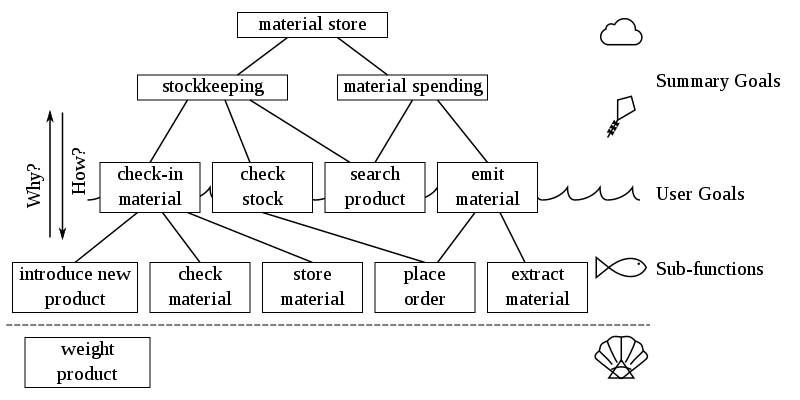
\includegraphics[width=1\textwidth]{./figures/chapter_02/09_cockburnstyle_use_cases.png}
        \setcaptioncitation{PENDIENTE}
        \caption{Niveles de los Objetivos}
        \label{fig:use_cases_levels}
      	\end{center}
      \end{figure}

      \item \textbf{Actor Principal \textit{(Principal Actor)}:} Indica al usuario que realiza o ejecuta el conjunto de acciones indicadas por el caso de usuario. Si bien Cockburn menciona en esta versión de caso de uso sólo un actor dentro del caso de uso, es posible incluir otros como actores secundarios.
      \item \textbf{\textit{Stakeholders} e intereses \textit{(Stakeholders and Interests)}:} Se atribuye al conjunto de stakeholder y los objetivos que cada uno busca.
      \item \textbf{Precondiciones \textit{(Preconditions)}:} Corresponden al conjunto de elementos que se deben cumplir antes de iniciar el flujo de etapas del caso de uso.
      \item \textbf{Estado de éxito \textit{(Success End Condition)}:} Muestra el estado en el cual el sistema se encuentra de la una ejecución exitosa del caso de uso.
      \item \textbf{Estado de error \textit{(Failed End Protection)}:} Describe el estado del sistema en caso de no alcanzar el objetivo.
      \item \textbf{\textit{Trigger}:} Corresponde a la acción que desencadena  el caso de uso.
      \item \textbf{Descripción \textit{(Description)}:} Conjunto de pasos a seguir para alcanzar el objetivo del caso de uso.
      \item \textbf{Extensiones \textit{(Extensions)}:} Corresponde a un flujo adicional que puede ser el caso de uso al momento de darse un condición especial sobre el sistema o los actores involucrados.
      \item \textbf{Variaciones \textit{(Variants)}:} Indica la ejecución de una misma acción de un modo distinto dentro del sistema , por ejemplo, al momento de pagar puede realizarse a través de dinero en efectivo, transferencia bancaria, entre otros.
    \end{enumerate}
\end{enumerate}

La lista anteriormente descrita puede verse resumida en el recuadro \ref{fig:uses_cases_summary} conocido por Cockburn \cite{uses_cases_writing} como la versión completamente vestida (fully dressed).

\begin{figure}[ht]
  \begin{center}
  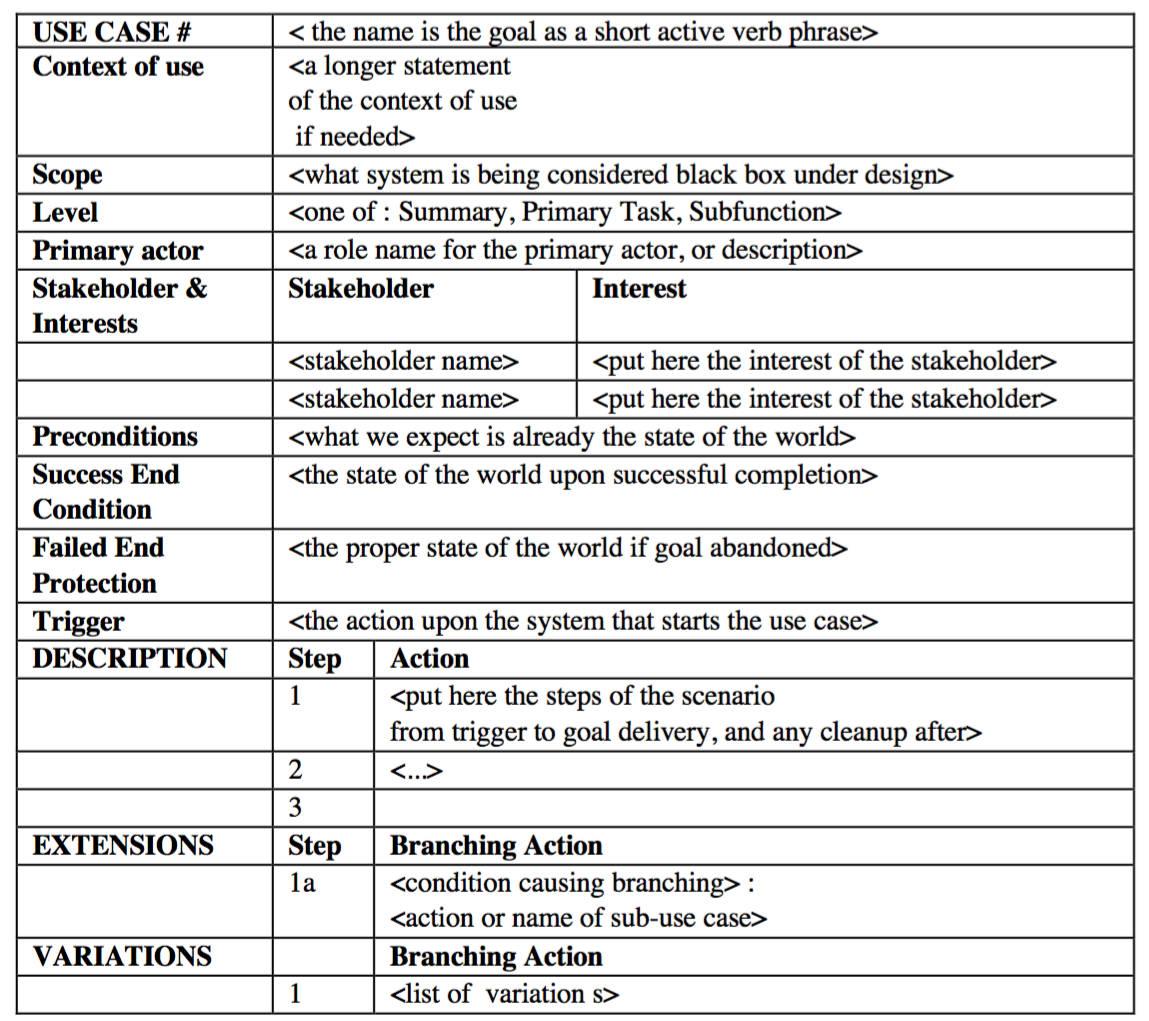
\includegraphics[width=0.8\textwidth]{./figures/chapter_02/10_use_case_template_one_column_version.png}
  \setcaptioncitation{PENDIENTE}
  \caption{Versión de Caso de Uso de una columna}
  \label{fig:uses_cases_summary}
  \end{center}
\end{figure}

Adicionalmente a lo descrito anteriormente, con el objetivo de tener una mejor visualización de la interacción entre casos de usos y actores principales como secundarios el \textit{Unified Modeling Language (U.M.L.)} \cite{uml} entrega los estándares y elementos para realizar la diagramación de un caso de uso. Este tipo de diagrama se denomina use case view o vista de un caso de uso. Los elementos presentes en esta visualización se aprecian en la representación gráfica de un caso de uso (figura \ref{fig:use_case_view}).

\begin{figure}[ht]
  \begin{center}
  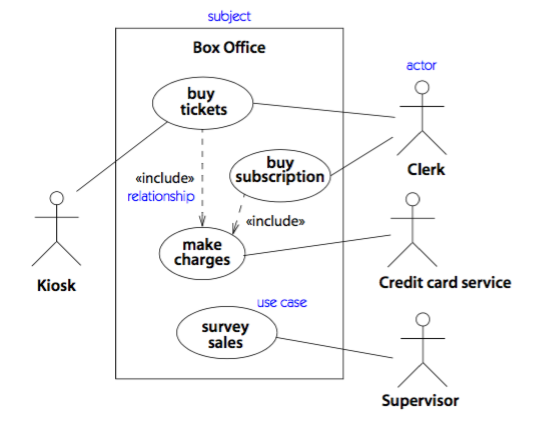
\includegraphics[width=0.8\textwidth]{./figures/chapter_02/11_use_case_view.png}
  \setcaptioncitation{PENDIENTE}
  \caption{Representación Gráfica de un Caso de Uso}
  \label{fig:use_case_view}
  \end{center}
\end{figure}

De este modo, para lograr la descripción de un caso de uso, se necesita tanto su diagrama descrito en UML como su detalle, el cual puede estar basado en la estructura propuesta por Cockburn o una estructura similar, pero más simple.

\subsubsection{Relatos de Usuarios \label{sec:user_stories}}

Según Mike Cohn \cite{user_stories_applied}, un relato de usuario describe una funcionalidad que es valorada por un usuario o otro sistema que se alimenta de ella.  Las partes de un relato consisten en la identificador,descripción de la funcionalidad, los criterios de aceptación, prioridad para el negocio y el puntaje de dificultad identificado por el equipo desarrollador. Adicional a lo anterior, cada relato de usuario debe cumplir las siguientes propiedades:

\begin{enumerate}
  \item \textbf{Independiente:} Un relato de usuario es independiente de los demás.
  \item \textbf{Negociable:} No son contratos , por lo que puede ser discutida y descrita por todos los \textit{stakeholders} y los miembros del equipo desarrollador.
  \item \textbf{Valorada por los compradores y por los usuarios:} Indica que las características del software descrito debe agregar valor tanto para las personas que lo ocupan como aquellas que “pagan” por él.
  \item \textbf{Estimable:} Es importante poder asignarle un tamaño al relato de usuario para identificar la cantidad de tiempo que tomará. Se indica que un relato que no es posible estimarlo es demasiado grande y es recomendable subdividirlo en varios.
  \item \textbf{Pequeña:} Indica que la descripción de un relato de un usuario no puede ser tan general porque en caso de ser así no podrá ser estimada de forma adecuada. En caso de suceder esto, se recomienda agruparlas bajo un epic \dictionary{epic} y que la funcionalidad  sea dividida en relatos de usuarios más pequeños y con mayor cantidad de detalle.
  \item \textbf{Comprobable:} Indica que debe existir una forma concreta y no general de que el relato de usuario se desarrolló de forma exitosa.
\end{enumerate}

Con el objetivo de que el relato de usuario pueda cumplir con las propiedades descritas anteriormente, Cohen recomienda utilizar el formato de tarjeta para su descripción. La siguiente imagen ilustra este concepto:

!!!!!! FIGURA !!!!!!

\begin{enumerate}
  \item \textbf{Identificador:} Compuesto por un número o nomenclatura con el formato US-XX, donde XX corresponde al número del relato.
  \item \textbf{Título:} Describe la funcionalidad que se debe desarrollador. El título debe posee el siguiente formato
    \begin{center}
      	As a \textbf{<type of user>}, I want \textbf{<some goal>} so that \textbf{<some reason>}.
    \end{center}

  Cohen \cite{user_stories_applied} indica que la parte <some reason> en muchos casos es opcional.
  \item \textbf{Puntaje:} Correspondiente al grado de dificultad del relato. Se espera que un relato de 2X tome el doble de tiempo que uno de X puntos.
  \item \textbf{Prioridad:} Indica el orden en el cual deben ser desarrolladas los relatos de usuarios.
  \item \textbf{Criterios de Aceptación:} Corresponde a las condiciones que debe cumplir el relato de usuario. No se especifica un formato para escribir un criterio de aceptación, pero se recomienda que indique de forma precisa lo que se espera del software, por ejemplo, el sistema debe solicitar el nombre, apellido y correo electrónico para poder identificar a un usuario.
\end{enumerate}

Otro punto importante que destaca Cohn es el uso de \textit{epics} \dictionary{epic}, él indica que no existe un criterio universal para clasificar una historia de usuario como grande, pero sí deben buscar cumplir del mejor modo las propiedades anteriormente descritas. Frente a la necesidad de agrupar, dos o más relatos de usuarios bajo un mismo concepto es cuando se hace el uso de un epic, el cual posee simplemente un nombre relativo a la funcionalidad que describe,una descripción para dar más contexto a quien lee la documentación del proyecto y un código identificador para realizar mejor el agrupamiento de los relatos de usuarios descritos anteriormente \cite{user_stories_applied}.

\subsection{Metodología y técnicas usadas en este trabajo \label{sec:work_decisions}}

Dentro de las metodologías y técnicas para levantamiento de requisitos descritas anteriormente para este proyecto se escogió la metodología XP y levantamiento de requisitos funcionales vía relatos de usuario. Se consideró que para la implementación de Scrum se hacía necesario incorporar un Product Owner, y un Scrum Master además de los miembros de equipo de desarrollo. XP es menos prescriptivo y permite organizar el  trabajo en función de la experiencia del equipo de desarrollo, siempre y cuando, se respeten los principios que ésta estipula.  Otro factor  que se tuvo en cuenta es que dada la considerable complejidad del problema, lo que buscábamos es más bien producir un primer prototipo o lo que se conoce como un \textit{Minimal Viable Product}, en adelante MVP \dictionary{mvp}. XP gracias a su principio  de simplicidad (Simplicity) permite abordar de mejor manera este escenario.

Por otro parte, a nivel de levantamiento de requisitos si bien tanto Casos de Usos como Relatos pueden ser aplicados con metodologías ágiles, se escogió relatos de usuario debido a su naturaleza menos estructurada que privilegia la comprensión de los requisitos en base a conversaciones con los  stakeholder Adicionalmente a lo anterior, las propiedades de los relatos de usuarios (independiente, negociable, valorado por los usuarios o compradores, estimable, pequeña y comprobable) permite un mejor registro de los esfuerzos invertidos en el desarrollo del prototipo.

Finalmente, el hecho de que el formato de los relatos de usuarios marque explícitamente el objetivo que se buscar resolver permite una mejor visualización general de las soluciones implementadas y al mismo tiempo permite llevar un control efectivo del avance del proyecto de modo más sencillo en base a cada uno de los artefactos requeridos por éste.

\section{Descubrimiento de Conocimiento (Knowledge Discovery) \label{sec:knowledge_discovery}}
Fayyad \cite{knowledge_discovery} en 1996 define término Knowledge Discovery como el conjunto de conocimientos relativos al proceso de extracción, almacenamiento y accesibilidad de datos; el uso de algoritmos ,en forma eficiente, para el análisis de los mismos; y, finalmente, la interpretación y visualización de resultados en base a estos, este resultado es conocido como \textit{knowledge}(conocimiento).

\subsection{Categorías, metodologías y modelos \label{sec:problem_categories}}
Desde la creación de este término hasta hoy en día han surgido varias metodologías para llevar a cabo el proceso anteriormente descrito, el cual se denomina \textit{Knowledge Discovery Process (KDP)}. Se logran logran identificar un total de 4 \cite{knowledge_discovery}:

\begin{enumerate}
  \item \textbf{\textit{Traditional KDP Approach}}\mbox{}\\ Agrupa aquellas metodologías que ocupan un proceso similar al propuesto por Fayyad et al., los cuales poseen las etapas de entendimiento del negocio, entendimiento de los datos, procesamientos de los datos, modelamiento o minería de datos, evaluación de modelos y ,finalmente, paso a producción o visualización. La característica principal de estas metodologías es que consisten en etapas secuenciales y sin mucha flexibilidad para la aceptación de cambios. La figura XX permite la visualización de estas etapas en funcionamiento:
  \item \textbf{\textit{Ontology-based KDP Approach}}\mbox{}\\ Se basa en la mezcla de ingeniería ontológica \dictionary{ontoligical} y un enfoque tradicional para KDP.
  \item \textbf{\textit{Web-based KDP Approach}} \mbox{} \\ Incorpora las mismas etapas que la primera categoría, pero reconoce de forma especial a la información proveniente de \textit{web logs} y ,por lo mismo, define etapas precisas para el tratamiento de la misma.
  \item \textbf{\textit{Agile-based KDP Approach}} \mbox{} \\  Esta categoría agrupa aquellos modelos que incorporan metodologías ágiles a un enfoque tradicional para KDP.
\end{enumerate}


\subsubsection{Modelos \label{sec:knowledge_discovery_models}}

Los mismos autores mencionados anteriormente, Mouhib y Asim, reconocen al mismo al mismo tiempos 9 modelos considerados líderes a lo largo de la historia de KDP, estos modelos son:

\begin{tabularx}{\linewidth}{@{}Y  Y  Y  Y@{}}
  \caption{Modelos a lo largo de la historia de \textit{KDP}} \label{tab:kdp_models}\\
  \toprule
  Nombre	&	Autor	&	Año de Creación
  \endhead
  \midrule
  Knowledge Discovery in Databases (KDD) Process & Fayyad et al. & 1996 \\
  \midrule
  Information Flow in a Data Mining Life Cycle & Ganesh et al. & 1996 \\
  \midrule
  SEMMA & SAS Institute & 1997 \\
  \midrule
  Refined KDD paradigm & Collier et al. & 1998 \\
  \midrule
  Knowledge Discovery Life Cycle (KDLC) Model & Lee and Kerschberg & 1998 \\
  \midrule
  CRoss-Industry-Standard Process for Data Mining (CRISP-DM) & CRISP-DM & 2000 \\
  \midrule
  Generic Data Mining Life Cycle by (DMLC) & Hofmann & 2003 \\
  \midrule
  Ontology Driven Knowledge Discovery Process (ODKD) & Gottgtroy & 2007 \\
  \midrule
  Adaptive Software Development-Data Mining (ASD-DM) Process Model & Alnoukari et al. & 2008 \\
\end{tabularx}

Dentro de todos los modelos mencionados anteriormente se consideran relevantes para el presente trabajo CRISP-DM y ASD-DM, los cuales se describen las siguientes secciones.

\subsubsection{CRISP-DM \label{crip_dm}}
Este fue uno de los primeros modelos que intentó abarcar la problema impuesta por el área de \textit{Knowledge Discovery}. Para lograr lo anterior este modelo define 4 niveles de abstracción, en los cuales se realizan actividades, las cuales a su vez pertenecen a una de las 6 fases específicas por las cuales pasa todo proceso. A continuación se ilustran los 4 niveles creados en este modelo:

!!!! FIGURA !!!!

Dentro de cada nivel se deben definir actividades, las cuales a su vez se encuentran categorizadas y divididas al mismo tiempo en sub tareas para poder llevarse a cabo. La intención de estos niveles jerárquicos es poder tener una clara agrupación de qué tareas específicas se realizan en cada proceso utilizada para la generación de conocimiento. Por otro lado, no existe un listado de actividades o tareas específicas que se deban realizar en cada uno de los niveles, sólo se espera que las tareas en las fases que se ilustran a continuación contengan sus tareas o actividades categorizadas en los niveles previamente mencionados.

!!!! FIGURA !!!!

Por la definición de estas fases se considera que este modelo posee un enfoque tradicional para KDP. Es posible establecer las siguientes definiciones para cada una de las fases ilustradas anteriormente \cite{knowledge_discovery}:

\begin{enumerate}
  \item \textbf{\textit{Business Understanding}:} Consiste en el entendimiento de los requerimientos generales del contexto en el cual se desenvuelve el proyecto así. En base a lo anterior, se crea una lista de objetivos que puedan ser respondidos por minería de datos y ,finalmente, elemento se crea una planificación general del proyecto.
  \item \textbf{\textit{Data Understanding}:} Esta etapa concierne específicamente a la recolección de los datos iniciales, descripción de ellos a través de metadata, exploración y verificación de la calidad de los mismos.
  \item \textbf{\textit{Data Preparation}:} Corresponden a todas las actividades necesarias para la creación del conjunto de datos final que será utilizada en la siguiente fase de modelamiento y análisis. Se encuentra dividido en : selección, limpieza, construcción, integración y formateo de datos.
  \item \textbf{\textit{Modeling}:} Orientado a la selección y aplicación apropiada de técnicas de modelamiento y minería de datos. Se encuentra seccionado en las fases de selección de técnicas de modelamiento, generación de pruebas, creación de modelos y ,finalmente, evaluación de los modelos generados.
  \item \textbf{\textit{Evaluation}:} Relacionado a la evaluar si el modelo escogido cumple con los objetivos impuestos en la primera fase.
  \item \textbf{\textit{Deployment}:} Etapa relacionada a la instalación a todo lo necesario para que el conocimiento generado puede ser ocupado por los usuarios finales. Esta etapa se caracteriza por presentar las siguientes fases: plan de instalación, plan de monitoreo y mantenimiento, generación de un reporte final donde se explica lo realizado y revisión de los pasos a seguir, en caso de ser requerido, de lo contrario, la finalización del proyecto.
\end{enumerate}

\subsubsection{Adaptative Software Development - Data Minning (ASD-DM) \label{asd_dm}}

Este modelo se caracteriza por la incorporación de elementos presentes en metodologías ágiles para los proyectos de minería de datos. La idea basal sobre esta filosofía es que un enfoque adaptativo (flexible y/o incremental) posee un mejor rendimiento al momento de trabajar con requerimientos desconocidos o cambiantes, efecto que no es posible resolver de forma eficiente en los enfoques tradicionales de KDP.

Para lograr su objetivo, este modelo \cite{knowledge_discovery} define 6 etapas organizadas en 3 fases que se muestran a continuación:

!!!!!! FIGURA !!!!!!!

Las etapas presentadas anteriormente pueden definirse del siguiente modo:

\begin{enumerate}
  \item \textbf{Etapa de Especulación \textit{(Speculation)}:} Incluye todas actividades que se necesiten realizar para el entendimiento del negocio y la preparación de los datos. Esta etapa termina cuando se han creado las fuentes de información en forma de \textit{data warehouse}, \textit{data marts}, cubos o agrupaciones de los datos.
  \item \textbf{Etapa de Colaboración \textit{(Collaboration)}:} Propicia toda actividad en donde se involucre a los stakeholders del proyecto para así poder escoger el mejor modelo para realizar la predicción posible.
  \item \textbf{Etapa de Aprendizaje \textit{(Learning)}:} Orientada a definir las tareas de pruebas y evaluación de los resultados obtenidos por el o los modelos escogidos en la fase anterior. En caso de ser los resultados aceptados por los \textit{stakeholders}, se procede a la entrega de un reporte final con los resultados explicados, de contrario, se vuelve a la fase anterior.
\end{enumerate}

\subsection{Metodologías y modelos usadas en este trabajo \label{sec:problem_categories}}

Si bien la metodología CRISP-DM presenta muchas de las cualidades que se necesitan para el desarrollo de este proyecto, no era la metodología más adecuada debido  a que incluye una claro paso a producción una vez que la etapa de evaluación haya llegado a su fin. El objetivo de este proyecto es poder presentar una primera solución al cálculo de la demanda de cursos del nuevo currículum de estudios, el cual aún no posee datos suficientes para poder realizar una generalización de datos para los próximos años. Frente a esta situación, se hace necesario que el proceso de aprendizaje se haga de un modo más continuo y que la nueva información que se vaya consiguiendo en el tiempo permita mejorar los niveles de predicción obtenidos. Teniendo en cuenta estos objetivos, se consideró que la metodología \textit{Adaptive Software Development-Data Mining} era la apropiada  gracias a la interacción continúa entre sus fases collaboration y learning, logrando así una incorporación de nuevos datos a medida que pase el tiempo e ir mejorando así los modelos predictivos creados.


\chapter[Capítulo 03]{Capítulo 03} \label{ch3}
\section{Introducción \label{sec:cap_three_introduction}}
El presente capítulo se encuentra orientado a la explicación de los objetivos detectados,de cómo las metodologías escogidas en el área de Ingeniería de Software y Descubrimiento del Conocimiento son utilizadas en el desarrollo de la solución y finalmente una descripción de los requerimientos levantados así como la descripción de los datos a utilizar para la realización de las estimaciones de demanda.

\section{Objetivos \label{sec:goals}}

Frente a la necesidad presentada de poder gestionar de forma adecuada la planificación de cursos y profesores dentro de la Escuela de Ingeniería en el contexto del nuevo curriculum, se identifica como objetivo principal calcular la cantidad de alumnos para un curso específico en el siguiente periodo académico, es decir, calcular la demanda para un curso en el siguiente semestre académico. Este objetivo plantea una serie de objetivos secundarios necesarios para el cumplimiento de éste. A continuación se enuncian estos objetivos secundarios para un mejor entendimiento del contexto en el cual se desenvuelve la problemática:

\section{Subsistemas y Metodología de Trabajo \label{sec:work_environment}}

\begin{enumerate}
	\item \textbf{Objetivo Principal:} Predecir en forma aproximada la demanda de alumnos para un curso específico en el siguiente semestre.
	\item \textbf{Objetivos Secundarios}
		\begin{enumerate}
			\item Tener una representación de la estructura de unidades académicas de la universidad en cada uno de sus niveles: escuelas e institutos.
			\item Apoyar en la gestión de los cursos del primer ciclo formativo (Licenciatura),  distribuidos en sus componentes básicas: plan de ciencias básicas, major y minor.
			\item Apoyar en la gestión de los majors y minors existentes así como la relación entre ellos.
			\item Apoyar en la gestión de cursos en las unidades académicas.
			\item Manejar la información histórica correspondiente al avance curricular por alumno en cada una de las generaciones.
			\item Evaluar diferentes estrategias de entrenamiento y predicción en los análisis predictivos de modo de  tener modelos actualizados.
			\item Visualizar las estimaciones históricas realizadas en base a la información que se posee.
		\end{enumerate}
\end{enumerate}

\subsection{Subsistemas \label{sec:sub_systems}}
Los objetivos planteados son respondidos mediante 3 grandes subsistemas:  una plataforma web que permite el almacenamiento de la información de histórica de los alumnos,  un conjunto de módulos para la creación de modelos predictivos y ua módulo de reportería que permite comparar los resultados para un curso en particular. La figura \ref{fig:subsystems} muestra los objetivos asociados a cada uno de estos subsistemas.

\begin{figure}[ht]
	\begin{center}
	  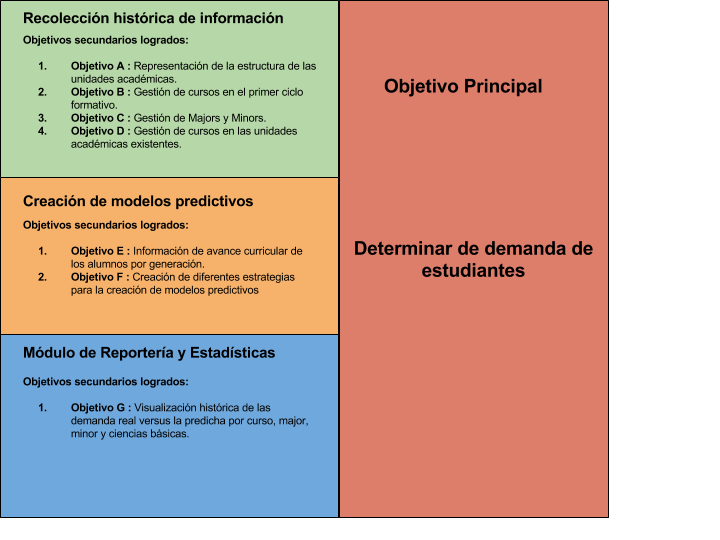
\includegraphics[width=0.8\textwidth]{./figures/chapter_03/01_objetivos.png}
	  \setcaptioncitation{Fuente Propia}
	  \caption{Subsistemas y sus objetivos}
	  \label{fig:subsystems}
	\end{center}
\end{figure}

\subsection{Metodología de trabajo \label{sec:work_methodology}}

La primera etapa incluye, por un lado, un levantamiento de los requerimientos funcionales, y por otro el análisis y preparación de los datos y utilizamos para ello métodos asociados a \textit{Extreme Programming (XP)} y \textit{Adaptive Software Development-Data Mining (ASD-DM)} respectivamente.   Los requerimientos funcionales quedan sintetizados en forma de relatos de usuario asociados a un conjunto de épicas.

Luego de la etapa inicial descrita anteriormente, se da inicio al proceso de desarrollo de software propiamente tal en forma iterativa e incremental, es decir, la creación sucesiva de pequeños entregables acumulativos usando un proceso iterativo de conversaciones con los \textit{stakeholders}. En paralelo con ello se lleva a cabo el proceso cíclico de modelación y evaluación de los algoritmos predictivos en \textit{ASDM-DM}.

\section{Requisitos \label{sec:requirements}}
\subsection{Usuarios \label{sec:user_description}}

La plataforma posee los siguientes tipos de usuarios o roles:

\begin{enumerate}
	\item \textbf{Administrador:} Manejo de usuarios, modelos predictivos, ejecuciones de entrenamiento y predicción, informes.
	\item \textbf{Estadístico:} Rol encargado de la mejora de los modelos estadístico, para ello puede solicitar entrenar modelos con diferentes estrategias y carga de modelos DSF en el sistema para un curso en particular. También posee la opción de realizar diferentes predicciones en un curso en particular o de todos los cursos cargados en el sistema.
	\item \textbf{Analista:} Puede correr nuevas predicciones y ver los resultados relativos a esas predicciones. Al mismo tiempo, puede ver la información acerca de los majors, minors, estudiantes y la historia de los mismos.
\end{enumerate}

\subsection{Épicas \label{sec:user_description}}

Las épicas corresponden a grupos de relatos de usuario que en forma conjunta permiten constituir una funcionalidad mayor. La siguiente lista muestra las épicas identificadas en este proyecto:

\begin{enumerate}
	\item \textbf{Administrador de Majors:} Permite la gestión de los majors dentro de la aplicación, es decir, la creación, eliminación , edición y la visualización dentro de la solución a implementarse. Adicionalmente, provee la posibilidad de administrar los cursos pertenecientes a cada major en particular.
	\item \textbf{Administrador de Minors:} Permite la gestión de los minors dentro de la aplicación, es decir, la creación, eliminación , edición y la visualización dentro de la solución a implementarse. Adicionalmente, provee la posibilidad de administrar los cursos pertenecientes a cada major en particular.
	\item \textbf{Carga de alumnos:} Corresponde a todas las funcionales que permiten la carga de información demográfica y de la universidad del alumno, tales como declaraciones de majors, minors, edad, generación, entre otras.
	\item \textbf{Carga de cursos:} Otorga la posibilidad de subir la información de los cursos y requisitos a través de un módulo de carga vía excel.
	\item \textbf{Carga de información histórica de un alumno:} Es el módulo encargado de validar y permite subir el avance curricular de los alumnos al sistema vía un archivo excel. Además, entrega indica cuando alguna información no entrega el formato esperado por el sistema.
	\item \textbf{Validar información de los cursos:} Conjunto de funcionalidades que permiten establecer el formato adecuado para la carga de los cursos de la universidad por unidad académica. Además, debe indicar el campo o los campos que no cumplen con el formato exigido.
	\item \textbf{Validar información de alumno:} Conjunto de funcionalidades que permiten establecer el formato adecuado para la carga de los alumnos. Además, debe indicar el campo o los campos que no cumplen con el formato exigido.
	\item \textbf{Validar información histórica de un alumno:} Conjunto de funcionalidades que permiten establecer el formato adecuado para el avance curricular de los alumnos. Además, debe indicar el campo o los campos que no cumplen con el formato exigido.
	\item \textbf{Laboratorio Predictivo:} Es la infraestructura y conjunto de funcionalidad que permite ejecutar modelos en el lenguaje de programación R, cuyos resultados son almacenados en la base de datos que utiliza el sistema.
	\item \textbf{Laboratorio de Entrenamiento:} Permite definir estrategias de entrenamiento sobre los datos históricos de los alumnos con el objetivo de poder mejorar la precisión de los modelos. Además, permite la gestión y almacenamiento de modelos en el formato RDS y \textit{scritps} \dictionary{script} del lenguaje R para la ejecución de modelos.
	\item \textbf{Otro:} Agrupa a todos aquellos relatos de usuarios que no encuentran en un epic anterior. Abarcan diferentes objetivos del software y ,por lo mismo, los relatos de usuarios no necesariamente presentan una correlación entre ellos.
\end{enumerate}

\subsection{Relatos de usuarios agrupados por Épicas \label{sec:detailed_user_stories}}

\subsubsection{Administrador de Majors}

\begin{enumerate}
	\item Relato 01
		\begin{enumerate}
			\item \textbf{Descripción:} Como administrador deseo desde el menú superior poder acceder a la opción Majors, así poder visualizar los majors creados en el sistema.
			\item \textbf{Criterios de aceptación}
				\begin{enumerate}
					\item Dado que ingresé a la sección Majors, el sistema me muestra una tabla paginada de los majors existentes en el sistema ordenados por fecha de creación. Los campos de la tabla corresponde a: nombre major y departamento al cual pertenecen.
					\item Dado que estoy la tabla paginada de los majors existentes, desde uno en particular es posible acceder al detalle de un major, eliminarlo. Al realizar la eliminación se elimina el major y las asociaciones respectivas con los cursos, sin eliminar estos últimos.
					\item Desde la tabla paginada, en la parte superior derecha existe un nuevo botón indicando \textbf{Nuevo Major}. El sistema despliega un formulario solicitando nombre y departamentos encargados.
				\end{enumerate}
		\end{enumerate}
	\item Relato 02
		\begin{enumerate}
			\item \textbf{Descripción:} Como un Administrador deseo poder visualizar el detalle de un major, el cual incluye un listado de cursos asociados al major indicando qué cursos son obligatorios y opcionales, así puedo visualizar el listado completo de cursos.
			\item \textbf{Criterios de aceptación}
				\begin{enumerate}
					\item Dado que ingresé al detalle de un major, la tabla paginada me muestra la sigla del curso, nombre,nombre del departamento cual lo dicta e indicando si el curso es obligatorio u opcional.
				\end{enumerate}
		\end{enumerate}
	\item Relato 03
		\begin{enumerate}
			\item \textbf{Descripción:} Como un Administrador deseo poder incorporar un nuevo curso a un major disponible en el sistema, así puedo administrar la estructura de los majors.
			\item \textbf{Criterios de aceptación}
				\begin{enumerate}
					\item Dado que estoy visualizando la tabla de cursos en el major, el sistema en la parte superior derecha de la tabla se podrá visualizar un botón que indica \textbf{Agregar Curso}.
					\item Dado incorporé un curso ya existente en la estructura, el sistema debe rechazar la incorporación de este.
				\end{enumerate}
		\end{enumerate}
	\item Relato 04
		\begin{enumerate}
			\item \textbf{Descripción:} Como un Estadístico deseo desde el menú superior poder acceder a la opción Majors, así poder visualizar los majors creados en el sistema.
			\item \textbf{Criterios de aceptación}
				\begin{enumerate}
					\item Dado que ingresé a la sección Majors, el sistema me muestra una tabla paginada de los majors existentes en el sistema ordenados por fecha de creación. Los campos de la tabla corresponde a: nombre major y departamento al cual pertenecen.
					\item Dado que estoy la tabla paginada de los majors existentes, desde uno en particular es posible acceder al detalle de un major, eliminarlo. Al realizar la eliminación se elimina el major y las asociaciones respectivas con los cursos, sin eliminar estos últimos.
				\end{enumerate}
		\end{enumerate}
	\item Relato 05
		\begin{enumerate}
			\item \textbf{Descripción:} Como un Estadístico deseo poder visualizar el detalle de un major, el cual incluye un listado de cursos asociados al major indicando qué cursos son obligatorios y opcionales, así puedo visualizar el listado completo de cursos.
			\item \textbf{Criterios de aceptación}
				\begin{enumerate}
					\item Dado que ingresé al detalle de un major, la tabla paginada me muestra la sigla del curso, nombre, nombre del departamento cual lo dicta e indicando si el curso es obligatorio u opcional.
				\end{enumerate}
		\end{enumerate}
	\item Relato 06
		\begin{enumerate}
			\item \textbf{Descripción:} Como un Estadístico deseo poder incorporar un nuevo curso a un major disponible en el sistema, así puedo administrar la estructura de los majors.
			\item \textbf{Criterios de aceptación}
				\begin{enumerate}
					\item Dado que estoy visualizando la tabla de cursos en el major, el sistema en la parte superior derecha de la tabla se podrá visualizar un botón que indica \textbf{Agregar Curso}.
					\item Dado incorporé un curso ya existente en la estructura, el sistema debe rechazar la incorporación de este.
				\end{enumerate}
		\end{enumerate}
\end{enumerate}

\subsubsection{Administrador de Minors}

\begin{enumerate}
	\item Relato 01
		\begin{enumerate}
			\item \textbf{Descripción:} Como un Administrador deseo desde el menú superior poder acceder a la opción Minors, así puedo reorganizar nuevos elementos dentro del minor.
			\item \textbf{Criterios de aceptación}
				\begin{enumerate}
					\item Dado que accedí a la opción Minors, se muestra una tabla pagina de los minors en el sistema, indicando nombre, fecha de creación y departamentos/facultades participantes en esté.
				\end{enumerate}
		\end{enumerate}
	\item Relato 02
		\begin{enumerate}
			\item \textbf{Descripción:} Como un Administrador deseo poder incorporar un nuevo curso a un minor disponible en el sistema, así puedo identificar el nivel de importancia del minor dentro de los estudiantes.
			\item \textbf{Criterios de aceptación}
				\begin{enumerate}
					\item Dado que estoy visualizando la lista de minors, en la parte superior derecha existe un botón que indica \textbf{Nuevo Minor}, al presionarlo se abre otra ventana con los datos en la tabla.
					\item Dado que estoy en el formulario de incorporación de cursos al minor, el curso debe existir previamente en el sistema. No es posible crearlo desde esta ventana.
					\item Dado que estoy en un formulario de asociación, el sistema debe consultar si el curso dentro del minor es optativo u obligatorio.
				\end{enumerate}
		\end{enumerate}
	\item Relato 03
		\begin{enumerate}
			\item \textbf{Descripción:} Como un Administrador deseo poder visualizar la estructura de cursos y alumnos han inscrito el minor, así puedo visualizar la cantidad total de minors en el sistema.
			\item \textbf{Criterios de aceptación}
				\begin{enumerate}
					\item Dado que estoy en la lista de minor disponibles en el sistema, en una columna existe una opción denominada \textbf{Ver detalle}, al hacer click en ella, el sistema me lleva a otra ventana donde se detalle una lista de los cursos pertenecientes al minor, alumnos que hay inscritos en él y un botón que indica \textbf{Incorporar curso}.
					\item Dado que estoy en la lista de cursos disponibles en el minor, al lado de cada curso existen las opciones de \textbf{desvincular} y cambiar estado de obligatorio a opcional y viceversa.
				\end{enumerate}
		\end{enumerate}
	\item Relato 04
		\begin{enumerate}
			\item \textbf{Descripción:} Como un Estadístico deseo desde el menú superior poder acceder a la opción Minors, así puedo reorganizar nuevos elementos dentro del minor.
			\item \textbf{Criterios de aceptación}
				\begin{enumerate}
					\item Dado que accedí a la opción Minors, se muestra una tabla página de los minors en el sistema, indicando nombre, fecha de creación y departamentos/facultades participantes en este.
				\end{enumerate}
		\end{enumerate}
	\item Relato 05
		\begin{enumerate}
			\item \textbf{Descripción:} Como un Estadístico deseo poder incorporar un nuevo curso a un minor disponible en el sistema, así puedo identificar el nivel de importancia del minor dentro de los estudiantes.
			\item \textbf{Criterios de aceptación}
				\begin{enumerate}
					\item Dado que estoy visualizando la lista de minors, en la parte superior derecha existe un botón que indica \textbf{Nuevo Minor}, al presionarlo se abre otra ventana con los datos en la tabla.
					\item Dado que estoy en el formulario de incorporación de cursos al minor, el curso debe existir previamente en el sistema. No es posible crearlo desde esta ventana.
					\item Dado que estoy en un formulario de asociación, el sistema debe consultar si el curso dentro del minor es optativo u obligatorio.
				\end{enumerate}
		\end{enumerate}
	\item Relato 06
		\begin{enumerate}
			\item \textbf{Descripción:} Como un Estadístico deseo poder visualizar la estructura de cursos y alumnos han inscrito el minor, así puedo mantener actualizado la información de los alumnos en el sistema.
			\item \textbf{Criterios de aceptación}
				\begin{enumerate}
					\item Dado que estoy en la lista de minor disponibles en el sistema, en una columna existe una opción denominada \textbf{Ver detalle}, al hacer click en ella, el sistema me lleva a otra ventana donde se detalle una lista de los cursos pertenecientes al minor, alumnos que hay inscritos en él y un botón que indica \textbf{"Incorporar curso"}.
					\item Dado que estoy en la lista de cursos disponibles en el minor, al lado de cada curso existen las opciones de \textbf{desvincular} y cambiar estado de obligatorio a opcional y viceversa.
				\end{enumerate}
		\end{enumerate}
\end{enumerate}

\subsubsection{Carga de alumnos}

\begin{enumerate}
	\item Relato 01
		\begin{enumerate}
			\item \textbf{Descripción:} Como un Administrador deseo poder carga un archivo excel con nuevos alumnos, así puedo ingresar nueva información histórica de alumnos
			\item \textbf{Criterios de aceptación}
				\begin{enumerate}
					\item Dado que ingresé a la sección alumnos, el sistema me muestra un formulario con la opción de de subir un archivo excel.
					\item Dado que visualicé el formulario para subir archivos, debajo de él existe una plantilla excel indicando los elementos y formato que se requieren. Los campos solicitados son rut, nombre, apellido paterno, apellido materno, generación, declaración de major a través de su código, declaración de minors a través de su código, major escogido a través de su código y minor a través de su código.
				\end{enumerate}
		\end{enumerate}
	\item Relato 02
		\begin{enumerate}
			\item \textbf{Descripción:} Como un Estadístico deseo poder carga un archivo excel con nuevos alumnos, así puedo ingresar nueva información histórica de alumnos.
			\item \textbf{Criterios de aceptación}
				\begin{enumerate}
					\item Dado que ingresé a la sección alumnos, el sistema me muestra un formulario con la opción de de subir un archivo excel.
					\item Dado que visualicé el formulario para subir archivos, debajo de él existe una plantilla excel indicando los elementos y formato que se requieren. Los campos solicitados son rut, nombre, apellido paterno, apellido materno, generación, declaración de major a través de su código, declaración de minors a través de su código, major escogido a través de su código y minor a través de su código.
				\end{enumerate}
		\end{enumerate}
	\item Relato 03
		\begin{enumerate}
			\item \textbf{Descripción:} Como un Analista deseo poder carga un archivo excel con nuevos alumnos, así puedo ingresar nueva información histórica de alumnos.
			\item \textbf{Criterios de aceptación}
				\begin{enumerate}
					\item Dado que ingresé a la sección alumnos, el sistema me muestra un formulario con la opción de de subir un archivo excel.
					\item Dado que visualicé el formulario para subir archivos, debajo de él existe una plantilla excel indicando los elementos y formato que se requieren. Los campos solicitados son rut, nombre, apellido paterno, apellido materno, generación, declaración de major a través de su código, declaración de minors a través de su código, major escogido a través de su código y minor a través de su código.
				\end{enumerate}
		\end{enumerate}
	\item Relato 04
		\begin{enumerate}
			\item \textbf{Descripción:} Como un Administrador deseo poder revisar las cargas de alumnos que se han realizado, así puedo llevar un control de los alumnos que se han ingresado al sistema.
			\item \textbf{Criterios de aceptación}
				\begin{enumerate}
					\item Dado que estoy en la página inicial, desde el menú Alumnos es posible obtener una opción para acceder a la cargas realizadas.
					\item Dado que hice click en la opción de cargas realizadas, el sistema me muestra una tabla paginada con el responsable, cantidad de alumnos y fecha de realización de la carga.
					\item Dado que ingresé al detalle de una carga, es posible tener la opción de eliminar la información de los alumnos subidos. Se borra toda la información relacionada, historial de cursos, predicciones realizadas.
				\end{enumerate}
		\end{enumerate}
	\item Relato 05
		\begin{enumerate}
			\item \textbf{Descripción:} Como un Estadístico deseo poder revisar las cargas de alumnos que se han realizado, así puedo llevar un control de los alumnos que se han ingresado al sistema.
			\item \textbf{Criterios de aceptación}
				\begin{enumerate}
					\item Dado que estoy en la página inicial, desde el menú Alumnos es posible obtener una opción para acceder a la cargas realizadas.
					\item Dado que hice click en la opción de cargas realizadas, el sistema me muestra una tabla paginada con el responsable, cantidad de alumnos y fecha de realización de la carga.
				\end{enumerate}
		\end{enumerate}
\end{enumerate}

\subsubsection{Carga de cursos}

\begin{enumerate}
	\item Relato 01
		\begin{enumerate}
			\item \textbf{Descripción:} Como un Administrador deseo poder cargar cursos a través de un archivo excel, así puedo ingresarlos al momento de que se creen en la UC.
			\item \textbf{Criterios de Aceptación}
				\begin{enumerate}
					\item Dado que me encuentro en la sección cursos, arriba de la tabla existe un formulario para ingresar un nuevo archivo excel.
					\item Dado que me encuentro en la sección cursos, debajo del formulario para subir nuevos cursos puedo descargar un archivo excel de plantilla para cumplir el formato requerido.
					\item Dado que ingresé un formulario completo, con datos correctos e hice click en el botón Cargar Cursos, en caso de que cumplan el formato, el sistema debe entregar un mensaje de éxito.
				\end{enumerate}
		\end{enumerate}
	\item Relato 02
		\begin{enumerate}
			\item \textbf{Descripción:} Como un Estadístico deseo poder cargar cursos a través de un archivo excel, asi puedo ingresarlos al momento de que se creen en la UC.
			\item \textbf{Criterios de Aceptación}
				\begin{enumerate}
					\item Dado que me encuentro en la sección cursos, arriba de la tabla existe un formulario para ingresar un nuevo archivo excel.
					\item Dado que me encuentro en la sección cursos, debajo del formulario para subir nuevos cursos puedo descargar un archivo excel de plantilla para cumplir el formato requerido.
					\item Dado que ingresé un formulario completo, con datos correctos e hice click en el botón Cargar Cursos, en caso de que cumplan el formato, el sistema debe entregar un mensaje de éxito.
				\end{enumerate}
		\end{enumerate}
	\item Relato 03
		\begin{enumerate}
			\item \textbf{Descripción:} Como un Analista deseo poder cargar cursos a través de un archivo excel, asi puedo ingresarlos al momento de que se creen en la UC.
			\item \textbf{Criterios de Aceptación}
				\begin{enumerate}
					\item Dado que me encuentro en la sección cursos, arriba de la tabla existe un formulario para ingresar un nuevo archivo excel.
					\item Dado que me encuentro en la sección cursos, debajo del formulario para subir nuevos cursos puedo descargar un archivo excel de plantilla para cumplir el formato requerido.
					\item Dado que ingresé un formulario completo, con datos correctos e hice click en el botón Cargar Cursos, en caso de que cumplan el formato, el sistema debe entregar un mensaje de éxito.
				\end{enumerate}
		\end{enumerate}
	\item Relato 04
		\begin{enumerate}
			\item \textbf{Descripción:} Como un Administrador deseo poder revisar la cargas que he realizado, así puedo llevar un seguimiento de qué cursos y cuándo se han cargado.
			\item \textbf{Criterios de Aceptación}
				\begin{enumerate}
					\item Desde el menú superior Cursos, el sistema me muestra la opción de acceder a historial de cargas.
					\item Dado que accedí al historial de descargar, el sistema me indica una tabla paginada indicando fecha de la carga de cursos, cantidad de cursos cargados y la opción para ver el detalle.
				\end{enumerate}
		\end{enumerate}
	\item Relato 05
		\begin{enumerate}
			\item \textbf{Descripción:} Como un Administrador deseo poder visualizar el detalle de una carga histórica, así puedo revisar de modo específico qué cursos se cargaron y quién fue el usuario que lo realizó.
			\item \textbf{Criterios de Aceptación}
				\begin{enumerate}
					\item Dado que presioné un click sobre la opción visualizar detalle desde la tabla página de historial de carga, el sistema me indica de modo general el usuario que realizó la carga, la cantidad de cursos cargados, la fecha de carga y una tabla paginada indicando los cursos subidos.
				\end{enumerate}
		\end{enumerate}
\end{enumerate}

\subsubsection{Carga de información histórica de un alumno}

\begin{enumerate}
	\item Relato 01
		\begin{enumerate}
			\item \textbf{Descripción:} Como un Administrador deseo poder información histórica de rendimiento de uno o varios a alumnos a través de un archivo excel, así puedo estar seguro de que el sistema usa la misma nomenclatura para la información histórica de alumnos.
			\item \textbf{Criterios de aceptación}
				\begin{enumerate}
					\item Dado que me encuentro en la lista de alumnos disponibles en el sistema, desde un lugar entre el menú superior y la tabla de los alumnos, exista un formulario donde se me da la opción de subir el archivo excel.
					\item Dado que estoy visualizando el formulario para el archivo excel, existe un link de descarga con la plantilla que puedo seguir. En ella se me indican los campos y formatos que debo seguir.
				\end{enumerate}
		\end{enumerate}
	\item Relato 02
		\begin{enumerate}
			\item \textbf{Descripción:} Como un Estadístico poder cargar la información histórica de rendimiento de uno o varios a alumnos a través de un archivo excel, así puedo estar seguro de que el sistema usa la misma nomenclatura para la información histórica de alumnos.
			\item \textbf{Criterios de aceptación}
				\begin{enumerate}
					\item Dado que me encuentro en la lista de alumnos disponibles en el sistema, desde un lugar entre el menú superior y la tabla de los alumnos, exista un formulario donde se me da la opción de subir el archivo excel.
					\item Dado que estoy visualizando el formulario para el archivo excel, existe un link de descarga con la plantilla que puedo seguir. En ella se me indican los campos y formatos que debo seguir.
				\end{enumerate}
		\end{enumerate}
	\item Relato 03
		\begin{enumerate}
			\item \textbf{Descripción:} Como un Analista deseo poder información histórica de rendimiento de uno o varios a alumnos a través de un archivo excel, así puedo estar seguro de que el sistema usa la misma nomenclatura para la información histórica de alumnos.
			\item \textbf{Criterios de aceptación}
				\begin{enumerate}
					\item Dado que me encuentro en la lista de alumnos disponibles en el sistema, desde un lugar entre el menú superior y la tabla de los alumnos, exista un formulario donde se me da la opción de subir el archivo excel.
					\item Dado que estoy visualizando el formulario para el archivo excel, existe un link de descarga con la plantilla que puedo seguir. En ella se me indican los campos y formatos que debo seguir.
				\end{enumerate}
		\end{enumerate}
\end{enumerate}

\subsubsection{Validar información de los cursos}

\begin{enumerate}
	\item Relato 01
		\begin{enumerate}
			\item \textbf{Descripción:} Como un Administrador deseo recibir un email cuando los cursos hayan sido validados y cargados en el sistema, así puedo asegurarme que la información cargada tenga la misma nomenclatura
			\item \textbf{Criterios de aceptación}
				\begin{enumerate}
					\item Dado que ingresé un excel al formulario con datos incorrectos, el sistema me debe indicar la línea y columna que no cumple con el formato requerido.
					\item Dado que ingresé un sigla ya existente, el sistema debe indicarme que no es posible crear este curso indicando fila y sigla existente.
					\item Dado que el ingresé una sigla, el nombre no puede estar vacío.
				\end{enumerate}
		\end{enumerate}
	\item Relato 02
		\begin{enumerate}
			\item \textbf{Descripción:} Como un Estadístico deseo recibir un email cuando los cursos hayan sido validados y cargados en el sistema, así puedo asegurarme que la información cargada tenga la misma nomenclatura
			\item \textbf{Criterios de aceptación}
				\begin{enumerate}
					\item Dado que ingresé un excel al formulario con datos incorrectos, el sistema me debe indicar la línea y columna que no cumple con el formato requerido.
					\item Dado que ingresé un sigla ya existente, el sistema debe indicarme que no es posible crear este curso indicando fila y sigla existente.
					\item Dado que el ingresé una sigla, el nombre no puede estar vacío.
				\end{enumerate}
		\end{enumerate}
	\item Relato 03
		\begin{enumerate}
			\item \textbf{Descripción:} Como un Analista deseo recibir un email cuando los cursos hayan sido validados y cargados en el sistema, así puedo asegurarme que la información cargada tenga la misma nomenclatura.
			\item \textbf{Criterios de aceptación}
				\begin{enumerate}
					\item Dado que ingresé un excel al formulario con datos incorrectos, el sistema me debe indicar la línea y columna que no cumple con el formato requerido.
					\item Dado que ingresé un sigla ya existente, el sistema debe indicarme que no es posible crear este curso indicando fila y sigla existente.
					\item Dado que el ingresé una sigla, el nombre no puede estar vacío.
				\end{enumerate}
		\end{enumerate}
\end{enumerate}

\subsubsection{Validar información de alumno}

\begin{enumerate}
	\item Relato 01
		\begin{enumerate}
			\item \textbf{Descripción:} Como un Administrador deseo poder recibir el resultado de la carga de nuevos alumnos vía email y en la pantalla del usuario, así verificar que se use la misma nomenclatura para todos los participantes del sistema.
			\item \textbf{Criterios de Aceptación:}
				\begin{enumerate}
					\item Dado que ingresé un archivo excel con información correcta, el sistema me indica un mensaje de éxito.
					\item Dado que ingresé un archivo excel con información incorrecta en formato, el sistema me indica la fila y columna e indicando que existe un error de formato. Además, indica cómo el campo debe ser completado.
					\item Dado que ingresé un archivo excel con información ya existente, el sistema me indica la fila y columna e indica cuál es la información duplicada.
				\end{enumerate}
		\end{enumerate}
	\item Relato 02
		\begin{enumerate}
			\item \textbf{Descripción:} Como un Estadístico deseo poder recibir el resultado de la carga de nuevos alumnos vía email y en la pantalla del usuario, así verificar que se use la misma nomenclatura para todos los participantes del sistema.
			\item \textbf{Criterios de Aceptación:}
				\begin{enumerate}
					\item Dado que ingresé un archivo excel con información correcta, el sistema me indica un mensaje de éxito.
					\item Dado que ingresé un archivo excel con información incorrecta en formato, el sistema me indica la fila y columna e indicando que existe un error de formato. Además, indica cómo el campo debe ser completado.
					\item Dado que ingresé un archivo excel con información ya existente, el sistema me indica la fila y columna e indica cuál es la información duplicada.
				\end{enumerate}
		\end{enumerate}
	\item Relato 03
		\begin{enumerate}
			\item \textbf{Descripción:} Como un Analista deseo poder recibir el resultado de la carga de nuevos alumnos vía email y en la pantalla del usuario, así verificar que se use la misma nomenclatura para todos los participantes del sistema.
			\item \textbf{Criterios de Aceptación:}
				\begin{enumerate}
					\item Dado que ingresé un archivo excel con información correcta, el sistema me indica un mensaje de éxito.
					\item Dado que ingresé un archivo excel con información incorrecta en formato, el sistema me indica la fila y columna e indicando que existe un error de formato. Además, indica cómo el campo debe ser completado.
					\item Dado que ingresé un archivo excel con información ya existente, el sistema me indica la fila y columna e indica cuál es la información duplicada.
				\end{enumerate}
		\end{enumerate}
\end{enumerate}

\subsubsection{Validar información histórica de un alumno}

\begin{enumerate}
	\item Relato 01
		\begin{enumerate}
			\item \textbf{Descripción:} Como un Administrador deseo poder saber que la información que incorporé en el excel se haya subido de forma exitosa, así puedo saber si se mantiene actualizada.
			\item \textbf{Criterios de Aceptación}
				\begin{enumerate}
					\item Dado que subí un excel con información correcta, el sistema me debe indicar los elementos fueron subidos de forma exitosa.
					\item Dado que subí un excel con información incorrecta, el archivo me debe indicar fila y columna del error, además indicar el tipo de error que existe. Pueden ser por formato o información ya existente.
				\end{enumerate}
		\end{enumerate}
	\item Relato 02
		\begin{enumerate}
			\item \textbf{Descripción:} Como un Estadístico deseo poder saber que la información que incorporé en el excel se haya subido de forma exitosa, así puedo saber si se mantiene actualizada.
			\item \textbf{Criterios de Aceptación}
				\begin{enumerate}
					\item Dado que subí un excel con información correcta, el sistema me debe indicar los elementos fueron subidos de forma exitosa.
					\item Dado que subí un excel con información incorrecta, el archivo me debe indicar fila y columna del error, además indicar el tipo de error que existe. Pueden ser por formato o información ya existente.
				\end{enumerate}
		\end{enumerate}
	\item Relato 03
		\begin{enumerate}
			\item \textbf{Descripción:} Como un Analista deseo poder saber que la información que incorporé en el excel se haya subido de forma exitosa, así puedo saber si se mantiene actualizada.
			\item \textbf{Criterios de Aceptación}
				\begin{enumerate}
					\item Dado que subí un excel con información correcta, el sistema me debe indicar los elementos fueron subidos de forma existosa.
					\item Dado que subí un excel con información incorrecta, el archivo me debe indicar fila y columna del error, además indicar el tipo de error que existe. Pueden ser por formato o información ya existente.
				\end{enumerate}
		\end{enumerate}
\end{enumerate}

\subsubsection{Laboratorio Predictivo}

\begin{enumerate}
	\item Relato 01
		\begin{enumerate}
			\item \textbf{Descripción:} Como un Administrador poder visualizar todos las predicciones realizadas en el sistema según tipo de predicción : curso, major,minor , departamento o conjunto de cursos., así puedo realizar análisis de modo granularidad por los tipo de predicciones realizadas.
			\item \textbf{Criterios de Aceptación}
				\begin{enumerate}
					\item Dado que inicié sesión, puedo visualizar un menú superior denominado Laboratorios y como submenú \textbf{Laboratorio predictivo}.
					\item Dado que hice click en la opción de \textbf{Laboratorio predictivo}, el sistema me dirige la página de las predicciones que se muestran en una tabla paginada indicando  nombre de la predicción, fecha de realización, tipo y botón de acciones. Las opciones son ver detalle y eliminar.
					\item Dado que hice click en eliminar, el sistema debe consultar si estoy seguro de querer realizarla. En caso de aceptar, se borra las predicciones realizadas y no los cursos y asociaciones entre alumnos.
				\end{enumerate}
		\end{enumerate}
	\item Relato 02
		\begin{enumerate}
			\item \textbf{Descripción:} Como un Administrador crear una nueva predicción indicando su nombre, tipo de predicción (curso, major, minor, departamento o conjunto de cursos), así puedo conocer un orden de magnitud de la cantidad de alumnos que tendrá el curso.
			\item \textbf{Criterios de Aceptación}
				\begin{enumerate}
					\item Dado que seleccioné tipo de evaluación curso, puedo seleccionar un curso en específico a través de un select.
					\item Dado que seleccioné tipo de evaluación major o minor, el sistema carga una lista de forma automática de los cursos de los cuales se hará una predicción.
					\item Dado que seleccioné tipo de evaluación departamento, el sistema carga de forma automática la lista de cursos que dicta el departamento.
				\end{enumerate}
		\end{enumerate}
	\item Relato 03
		\begin{enumerate}
			\item \textbf{Descripción:} Como un Administrador poder visualizar el resultado de la predicción por cursos al hacer click en \textbf{detalle} desde la tabla de predicciones realizadas, así puedo realizar visualizar si puedo realizar una predicción de forma correcta por tipo de predicción (curso, major, minor, departamento o conjunto de cursos).
			\item \textbf{Criterios de Aceptación}
				\begin{enumerate}
					\item Dado que realicé la predicción, los detalles esperado son : cantidad de alumnos por curso. En caso de existir más de un curso, se espera tener una tabla paginada ordenada por sigla de cada uno.
				\end{enumerate}
		\end{enumerate}
\end{enumerate}

\subsubsection{Laboratorio de Entrenamiento}

\begin{enumerate}
	\item Relato 01
		\begin{enumerate}
			\item \textbf{Descripción:} Como un Administrador poder visualizar todos los cursos que tienen asignado un modelo predictivo , así poder visualizar si el curso está listo para poder realizar un predicción de la cantidad de alumnos a tomar el próximo semestre.
			\item \textbf{Criterios de Aceptación}
				\begin{enumerate}
					\item Dado que inicié sesión, en la barra superior puedo acceder al menú \textbf{Laboratorio} y como submenu \textbf{Laboratorio de entrenamiento}.
					\item Dado que hice click en la opción \textbf{Laboratorio de entrenamiento}, puedo visualizar una lista de cursos en una tabla con el siguiente detalle : Sigla del curso, nombre del curso, estado (indica si posee  o no un modelo predictivo cargado) y acciones, indicando ver detalle, cargar modelo, carga script de ejecución, carga script de entrenamiento y eliminar. (Los script cargados deben ser en código R).
					\item Dado que seleccioné la opción eliminar, el sistema me indica un mensaje indicando si estoy seguro de hacerlo. En caso afirmativo, el sistema borra el script de ejecución del modelo junto al modelo cargado.
				\end{enumerate}
		\end{enumerate}
	\item Relato 02
		\begin{enumerate}
			\item \textbf{Descripción:} Como un Administrador poder visualizar el detalle de un curso en el laboratorio predictivo, así puedo estar seguro de que mi modelo se está entrenando con una buena calidad.
			\item \textbf{Criterios de Aceptación}
				\begin{enumerate}
					\item Dado que hice click en la parte \textbf{detalle} de la lista de cursos en el laboratorio predictivo, el sistema me lleva a una página indicando sigla, nombre y departamento que lo dicta (en caso de ser un curso en conjunto, se muestra la lista de los departamentos), checklist de scripts cargados o creados para el o los cursos indicando si el script de predicción, entrenamiento y modelo se encuentran creados.
					\item Dado que me encuentro en el detalle un curso en el laboratorio de entrenamiento, puedo visualizar una tabla con los entrenamientos realizados en el curso. Al momento de realizar un entrenamiento, se crea el modelo como un archivo RDS (en caso de uno existente, crea una nueva versión del archivo). La opción para crear un nuevo entrenamiento se encuentra en la parte superior de todos los realizados.
				\end{enumerate}
		\end{enumerate}
	\item Relato 03
		\begin{enumerate}
			\item \textbf{Descripción:} Como un Administrador poder realizar un nuevo entrenamiento a un curso en particular definiendo el porcentaje para el set de entrenamiento, validación y regularización (evitar overfitting). , así puedo evaluar qué modelo predice mejor.
			\item \textbf{Criterios de Aceptación}
				\begin{enumerate}
					\item Dado que deseo crea un nuevo entrenamiento, debo definir los porcentajes para cada tipo de set de datos (entrenamiento, validación y regularización) y la semilla para organizar de forma random los elementos del set de entrenamiento.
					\item Dado que se ha creado una predicción, se crea una nueva versión de los archivos de ejecución, entrenamiento y modelo.
				\end{enumerate}
		\end{enumerate}
	\item Relato 04
		\begin{enumerate}
			\item \textbf{Descripción:} Como un Administrador poder crear comparación de estrategias seleccionando diferentes porcentajes para los de entrenamiento y validación.
			\item \textbf{Criterios de Aceptación}
				\begin{enumerate}
					\item Dado que apreté nueva predicción para un curso determinado, debo seleccionar qué tipo de entrenamiento será: simple o comparativo. En el primer caso se solicita sólo una vez los porcentajes para los sets de datos, en el segundo, dos veces para realizar la comparación.
					\item Dado que realicé una predicción, su detalle entrega la matriz de confusión de los datos, así como también las siguientes medidas de error rate, accurary, recall y sensivity.
				\end{enumerate}
		\end{enumerate}
\end{enumerate}

\subsubsection{Otro}

\begin{enumerate}
	\item Relato 01
		\begin{enumerate}
			\item \textbf{Descripción:} Como un Administrador poder ingresar al sistema usando mi email uc o de ingeniería, puedo acceder a todos los modelos del sistema.
			\item \textbf{Criterios de Aceptación}
				\begin{enumerate}
					\item Dado que tengo una cuenta en el sistema , debería ser capaz de acceder usando mi email y password.
					\item Dado que ingresé un email no válido para el sistema, debe indicarse que el email no existe.
					\item Dado que ingresé un texto en el campo email que no cumplía con el formato, se debe mostrar un mensaje de error.
				\end{enumerate}
		\end{enumerate}
	\item Relato 02
		\begin{enumerate}
			\item \textbf{Descripción:} Como un Analista poder ingresar al sistema usando mi email uc o de ingeniería, puedo acceder a todos los modelos del sistema.
			\item \textbf{Criterios de Aceptación}
				\begin{enumerate}
					\item Dado que recibí un email de creación de cuenta, debería ser capaz de acceder usando mi email y password.
					\item Dado que ingresé un email no válido para el sistema, debe indicarse que el email no existe.
					\item Dado que ingresé un texto en el campo email que no cumplía con el formato, se debe mostrar un mensaje de error.
				\end{enumerate}
		\end{enumerate}
	\item Relato 03
		\begin{enumerate}
			\item \textbf{Descripción:} Como un Estadístico poder ingresar al sistema usando mi email uc o de ingeniería, puedo acceder a todos los modelos del sistema.
			\item \textbf{Criterios de Aceptación}
				\begin{enumerate}
					\item Dado que recibí un email de creación de cuenta, debería ser capaz de acceder usando mi email y password.
					\item Dado que ingresé un email no válido para el sistema, debe indicarse que el email no existe.
					\item Dado que ingresé un texto en el campo email que no cumplía con el formato, se debe mostrar un mensaje de error.
				\end{enumerate}
		\end{enumerate}
	\item Relato 04
		\begin{enumerate}
			\item \textbf{Descripción:} Como un Administrador deseo poder recuperar mi contraseña recibiendo un email al email asociado a la cuenta creada.
			\item \textbf{Criterios de Aceptación}
				\begin{enumerate}
					\item Dado que tengo mi cuenta creada, debería ser capaz de enviarme un email de recuperación de contraseña a través de un link.
					\item Dado que recibí el email para cambiar mi contraseña e hice click en el link antes de las 24 hrs de su expiración, debería poder escoger una nueva contraseña con validación para ingresar nuevamente.
				\end{enumerate}
		\end{enumerate}
	\item Relato 05
		\begin{enumerate}
			\item \textbf{Descripción:} Como un Estadístico deseo poder recuperar mi contraseña recibiendo un email al email asociado a la cuenta creada.
			\item \textbf{Criterios de Aceptación}
				\begin{enumerate}
					\item Dado que tengo mi cuenta creada, debería ser capaz de enviarme un email de recuperación de contraseña a través de un link.
					\item Dado que recibí el email para cambiar mi contraseña e hice click en el link antes de las 24 hrs de su expiración, debería poder escoger una nueva contraseña con validación para ingresar nuevamente.
				\end{enumerate}
		\end{enumerate}
	\item Relato 06
		\begin{enumerate}
			\item \textbf{Descripción:} Como un Estadístico deseo poder recuperar mi contraseña recibiendo un email al email asociado a la cuenta creada.
			\item \textbf{Criterios de Aceptación}
				\begin{enumerate}
					\item Dado que tengo mi cuenta creada, debería ser capaz de enviarme un email de recuperación de contraseña a través de un link.
					\item Dado que recibí el email para cambiar mi contraseña e hice click en el link antes de las 24 hrs de su expiración, debería poder escoger una nueva contraseña con validación para ingresar nuevamente.
				\end{enumerate}
		\end{enumerate}
	\item Relato 07
		\begin{enumerate}
			\item \textbf{Descripción:} Como un Administrador deseo poder manejar a los usuarios dentro del sistema que no sea administradores, así puedo corregir problemas relacionados a su información o interacción en el sistema.
			\item \textbf{Criterios de Aceptación}
				\begin{enumerate}
					\item Dado que inicie sesión como administrador, mi primera vista debe ser una lista página de los usuarios disponibles indicando nombre, apellido, email y rol.
					\item Dado que tengo privilegios de administrador, puedo resetear la contraseña de un usuario ya sea ingresando una nueva con verificación o enviándole un email para que él lo haga.
					\item Dado que tengo privilegios de administrador, puede deshabilitar un usuario sin borrar su cuenta (soft delete).
				\end{enumerate}
		\end{enumerate}
	\item Relato 08
		\begin{enumerate}
			\item \textbf{Descripción:} Como un Administrador deseo poder visitar la sección cursos, así puedo gestionar los cursos existentes.
			\item \textbf{Criterios de Aceptación}
				\begin{enumerate}
					\item Dado que ingrese a la sección desde el menú superior, debo poder visualizar todos los cursos ingresados al sistema en una lista página indicando nombre del curso , sigla, descripción y programa.
					\item Dado que estoy en sección cursos, en la lista paginada cada curso tiene la opción de visitar detalles, cambiar su estado (habilitado/deshabilitado). La opción eliminar queda habilitada sólo para el administrador.
				\end{enumerate}
		\end{enumerate}
	\item Relato 09
		\begin{enumerate}
			\item \textbf{Descripción:} Como un Analista deseo poder visitar la sección cursos, así puedo gestionar los cursos existentes.
			\item \textbf{Criterios de Aceptación}
				\begin{enumerate}
					\item Dado que ingrese a la sección desde el menú superior, debo poder visualizar todos los cursos ingresados al sistema en una lista pagina indicando nombre del curso , sigla, descripción y programa.
					\item Dado que estoy en sección cursos, en la lista paginada cada curso tiene la opción de visitar detalles, cambiar su estado (habilitado/deshabilitado). La opción eliminar queda habilitada sólo para el administrador.
				\end{enumerate}
		\end{enumerate}
	\item Relato 10
		\begin{enumerate}
			\item \textbf{Descripción:} Como un Estadístico deseo poder visitar la sección cursos, así puedo gestionar los cursos existentes.
			\item \textbf{Criterios de Aceptación}
				\begin{enumerate}
					\item Dado que ingrese a la sección desde el menú superior, debo poder visualizar todos los cursos ingresados al sistema en una lista página indicando nombre del curso , sigla, descripción y programa.
					\item Dado que estoy en sección cursos, en la lista paginada cada curso tiene la opción de visitar detalles, cambiar su estado (habilitado/deshabilitado). La opción eliminar queda habilitada sólo para el administrador.
				\end{enumerate}
		\end{enumerate}
	\item Relato 11
		\begin{enumerate}
			\item \textbf{Descripción:} Como un Administrador deseo poder revisar alumnos en el sistema, así puedo realizar un seguimiento si la información de alumnos se encuentra actualizada en el sistema.
			\item \textbf{Criterios de Aceptación}
				\begin{enumerate}
					\item Dado que ingresé a la opción alumnos, el sistema me muestra un resumen indicando la cantidad de alumnos por generación y una tabla paginada de los alumnos ordenados por fecha de creación.
					\item Dado que me encuentro en el menú superior, me indica la opción \textbf{Alumnos}.
				\end{enumerate}
		\end{enumerate}
	\item Relato 12
		\begin{enumerate}
			\item \textbf{Descripción:} Como un Administrador deseo poder visualizar la información histórica de un alumnos en particular, así puedo mantener actualizado la información de los alumnos en el sistema.
			\item \textbf{Criterios de Aceptación}
				\begin{enumerate}
					\item Dado que estoy en la sección \textbf{Alumnos}, desde la tabla de alumnos paginada existe la opción ver detalle. En el detalle se indica nombre, apellido, declaración de major, declaración de minor, lista de cursos tomados junto a su respectivos resultados.
				\end{enumerate}
		\end{enumerate}
	\item Relato 13
		\begin{enumerate}
			\item \textbf{Descripción:} Como un Estadístico deseo poder visualizar la información histórica de un alumno en particular, así puedo mantener actualizado la información de los alumnos en el sistema.
			\item \textbf{Criterios de Aceptación}
				\begin{enumerate}
					\item Dado que estoy en la sección \textbf{Alumnos}, desde la tabla de alumnos paginada existe la opción ver detalle. En el detalle se indica nombre, apellido, declaración de major, declaración de minor, lista de cursos tomados junto a su respectivos resultados.
				\end{enumerate}
		\end{enumerate}
	\item Relato 14
		\begin{enumerate}
			\item \textbf{Descripción:} Como un Analista deseo poder visualizar la información histórica de un alumnos en particular, así puedo llevar un control de todos los cursos que se han realizado una predicción.
			\item \textbf{Criterios de Aceptación}
				\begin{enumerate}
					\item Dado que estoy en la sección \textbf{Alumnos}, desde la tabla de alumnos paginada existe la opción ver detalle. En el detalle se indica nombre, apellido, declaración de major, declaración de minor, lista de cursos tomados junto a su respectivos resultados.
				\end{enumerate}
		\end{enumerate}
\end{enumerate}


\subsection{Requisitos No Funcionales \label{sec:user_description}}

\subsubsection{Rendimiento \label{sec:performance}}

	\begin{enumerate}
		\item El sistema debe indicar en no más de 1 segundo que ha iniciado ha procesar la solicitud de predicción de los modelos predictivos.
		\item El sistema debe demorarse a lo más 12 hrs en procesar su predicción más compleja, en caso de no hacerlo, debe informar al usuario los motivos.
	\end{enumerate}

\subsubsection{Escalamiento \label{sec:scalability}}

	\begin{enumerate}
		\item El sistema debe soportar la solicitud de una predicción ya sea para un curso o conjunto de ellos en cualquier instante.
		\item Para lograr mejoras en los procesamiento de las predicciones, el sistema ejecuta cada predicción de forma independiente en servers configurados en el sistema.
	\end{enumerate}

\subsubsection{Usabilidad \label{sec:usability}}
	\begin{enumerate}
		\item El sistema usa el framework Bootstrap para lograr un estándar básico de diseño.
		\item Se realiza una prueba de usabilidad con los usuarios finales utilizando el manual del sistema, el cual contempla desde la carga de los datos hasta la visualización del resultado de un modelo predictivo.
	\end{enumerate}

\section{Arquitectura \label{sec:architecture}}
\subsection{Diagrama de Contexto \label{sec:context_diagram}}

	\begin{figure}[H]
		\begin{center}
		  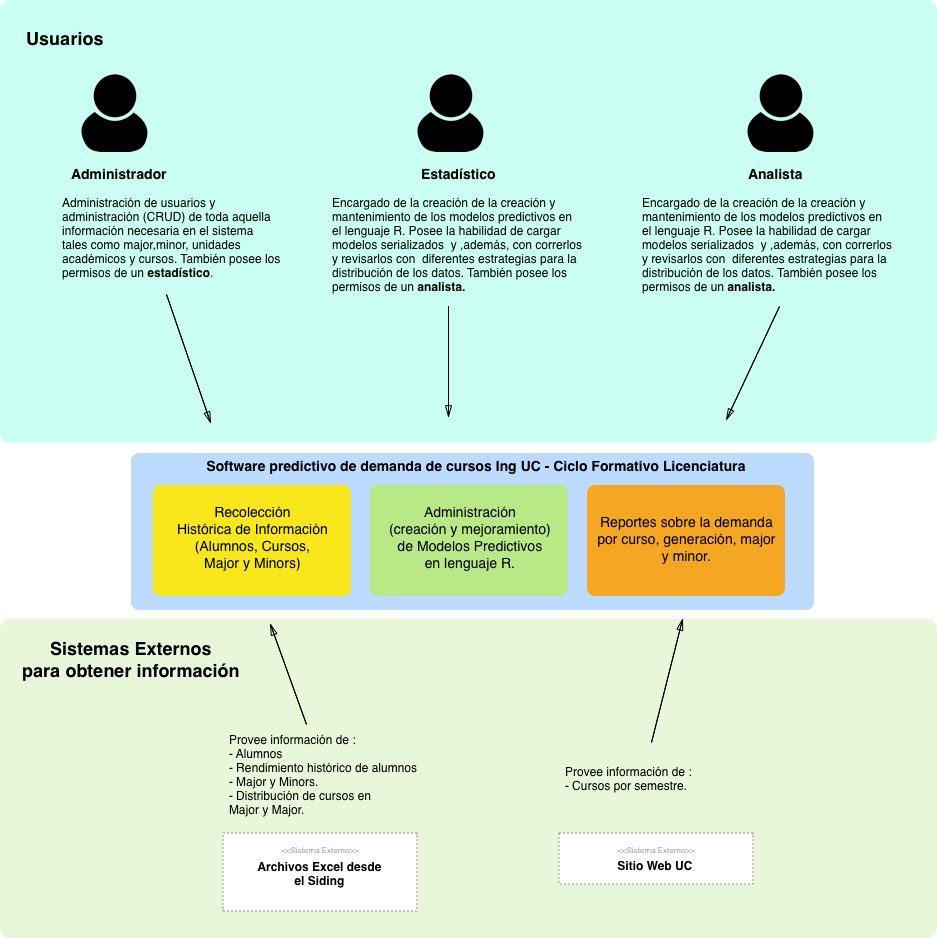
\includegraphics[width=0.95\textwidth]{./figures/chapter_03/02_diagrama_de_contexto.png}
		  \setcaptioncitation{Fuente Propia}
		  \caption{Diagrama de Contexto}
		  \label{fig:context_diagram_picture}
		\end{center}
	\end{figure}


\subsection{Diagrama de Componentes \label{sec:components_diagram}}

	\begin{figure}[H]
		\begin{center}
			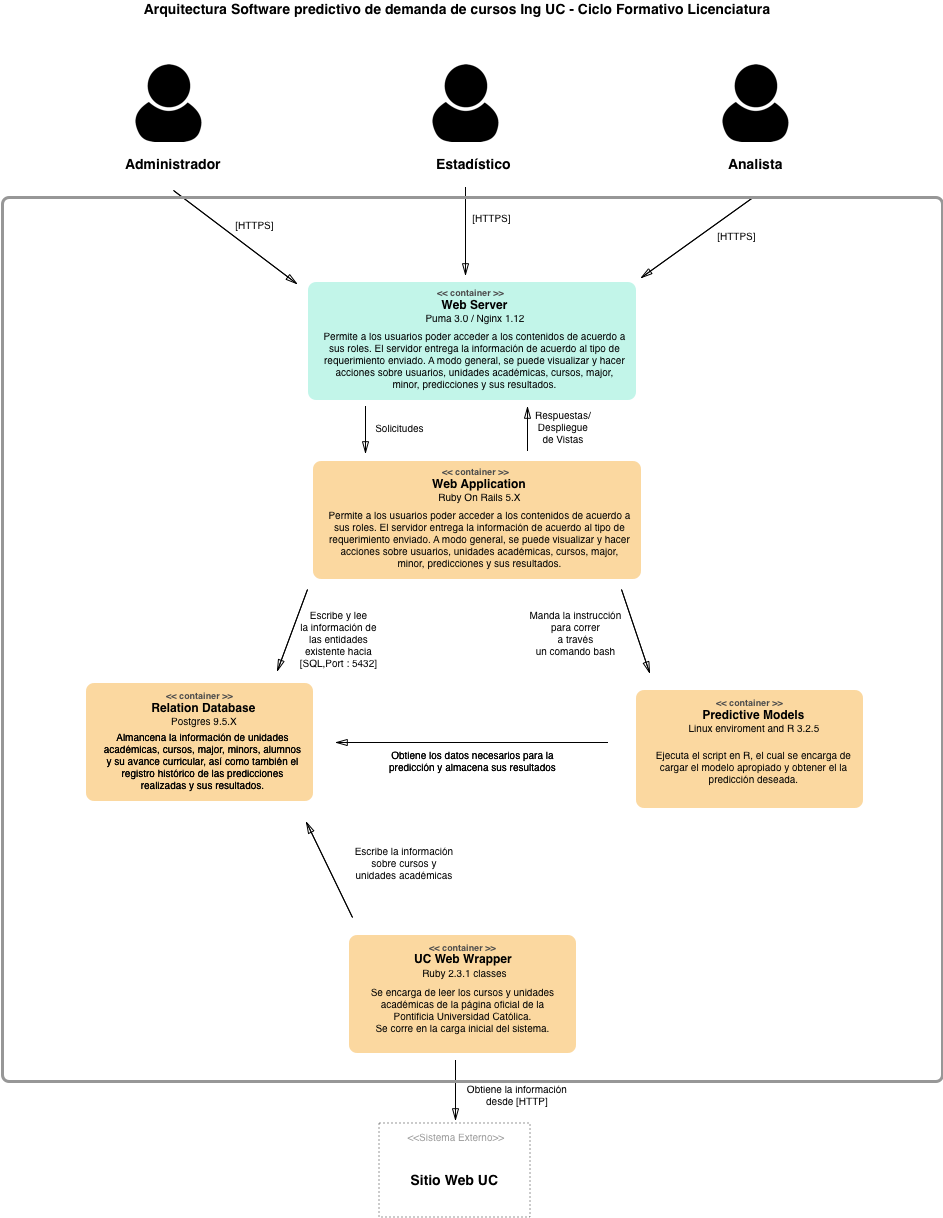
\includegraphics[width=0.9\textwidth]{./figures/chapter_03/03_diagrama_de_componentes.png}
			\setcaptioncitation{Fuente Propia}
			\caption{Diagrama de Componentes}
			\label{fig:components_diagram_picture}
		\end{center}
	\end{figure}


\subsection{Descripción de los Datos \label{sec:data_description}}

En las siguientes secciones se describen el conjunto datos y su estructura para realizar las predicciones de demanda de los cursos. En la primera parte se describe el modelo de base de datos utilizado y ,a continuación, el procedimiento de de cómo debe ir alimentándose el software para crear mantener la consistencia de la información.

\subsubsection{Modelo de datos \label{sec:data_model}}

El modelo de datos de la solución a implementar es el siguiente:

	\begin{figure}[H]
		\begin{center}
			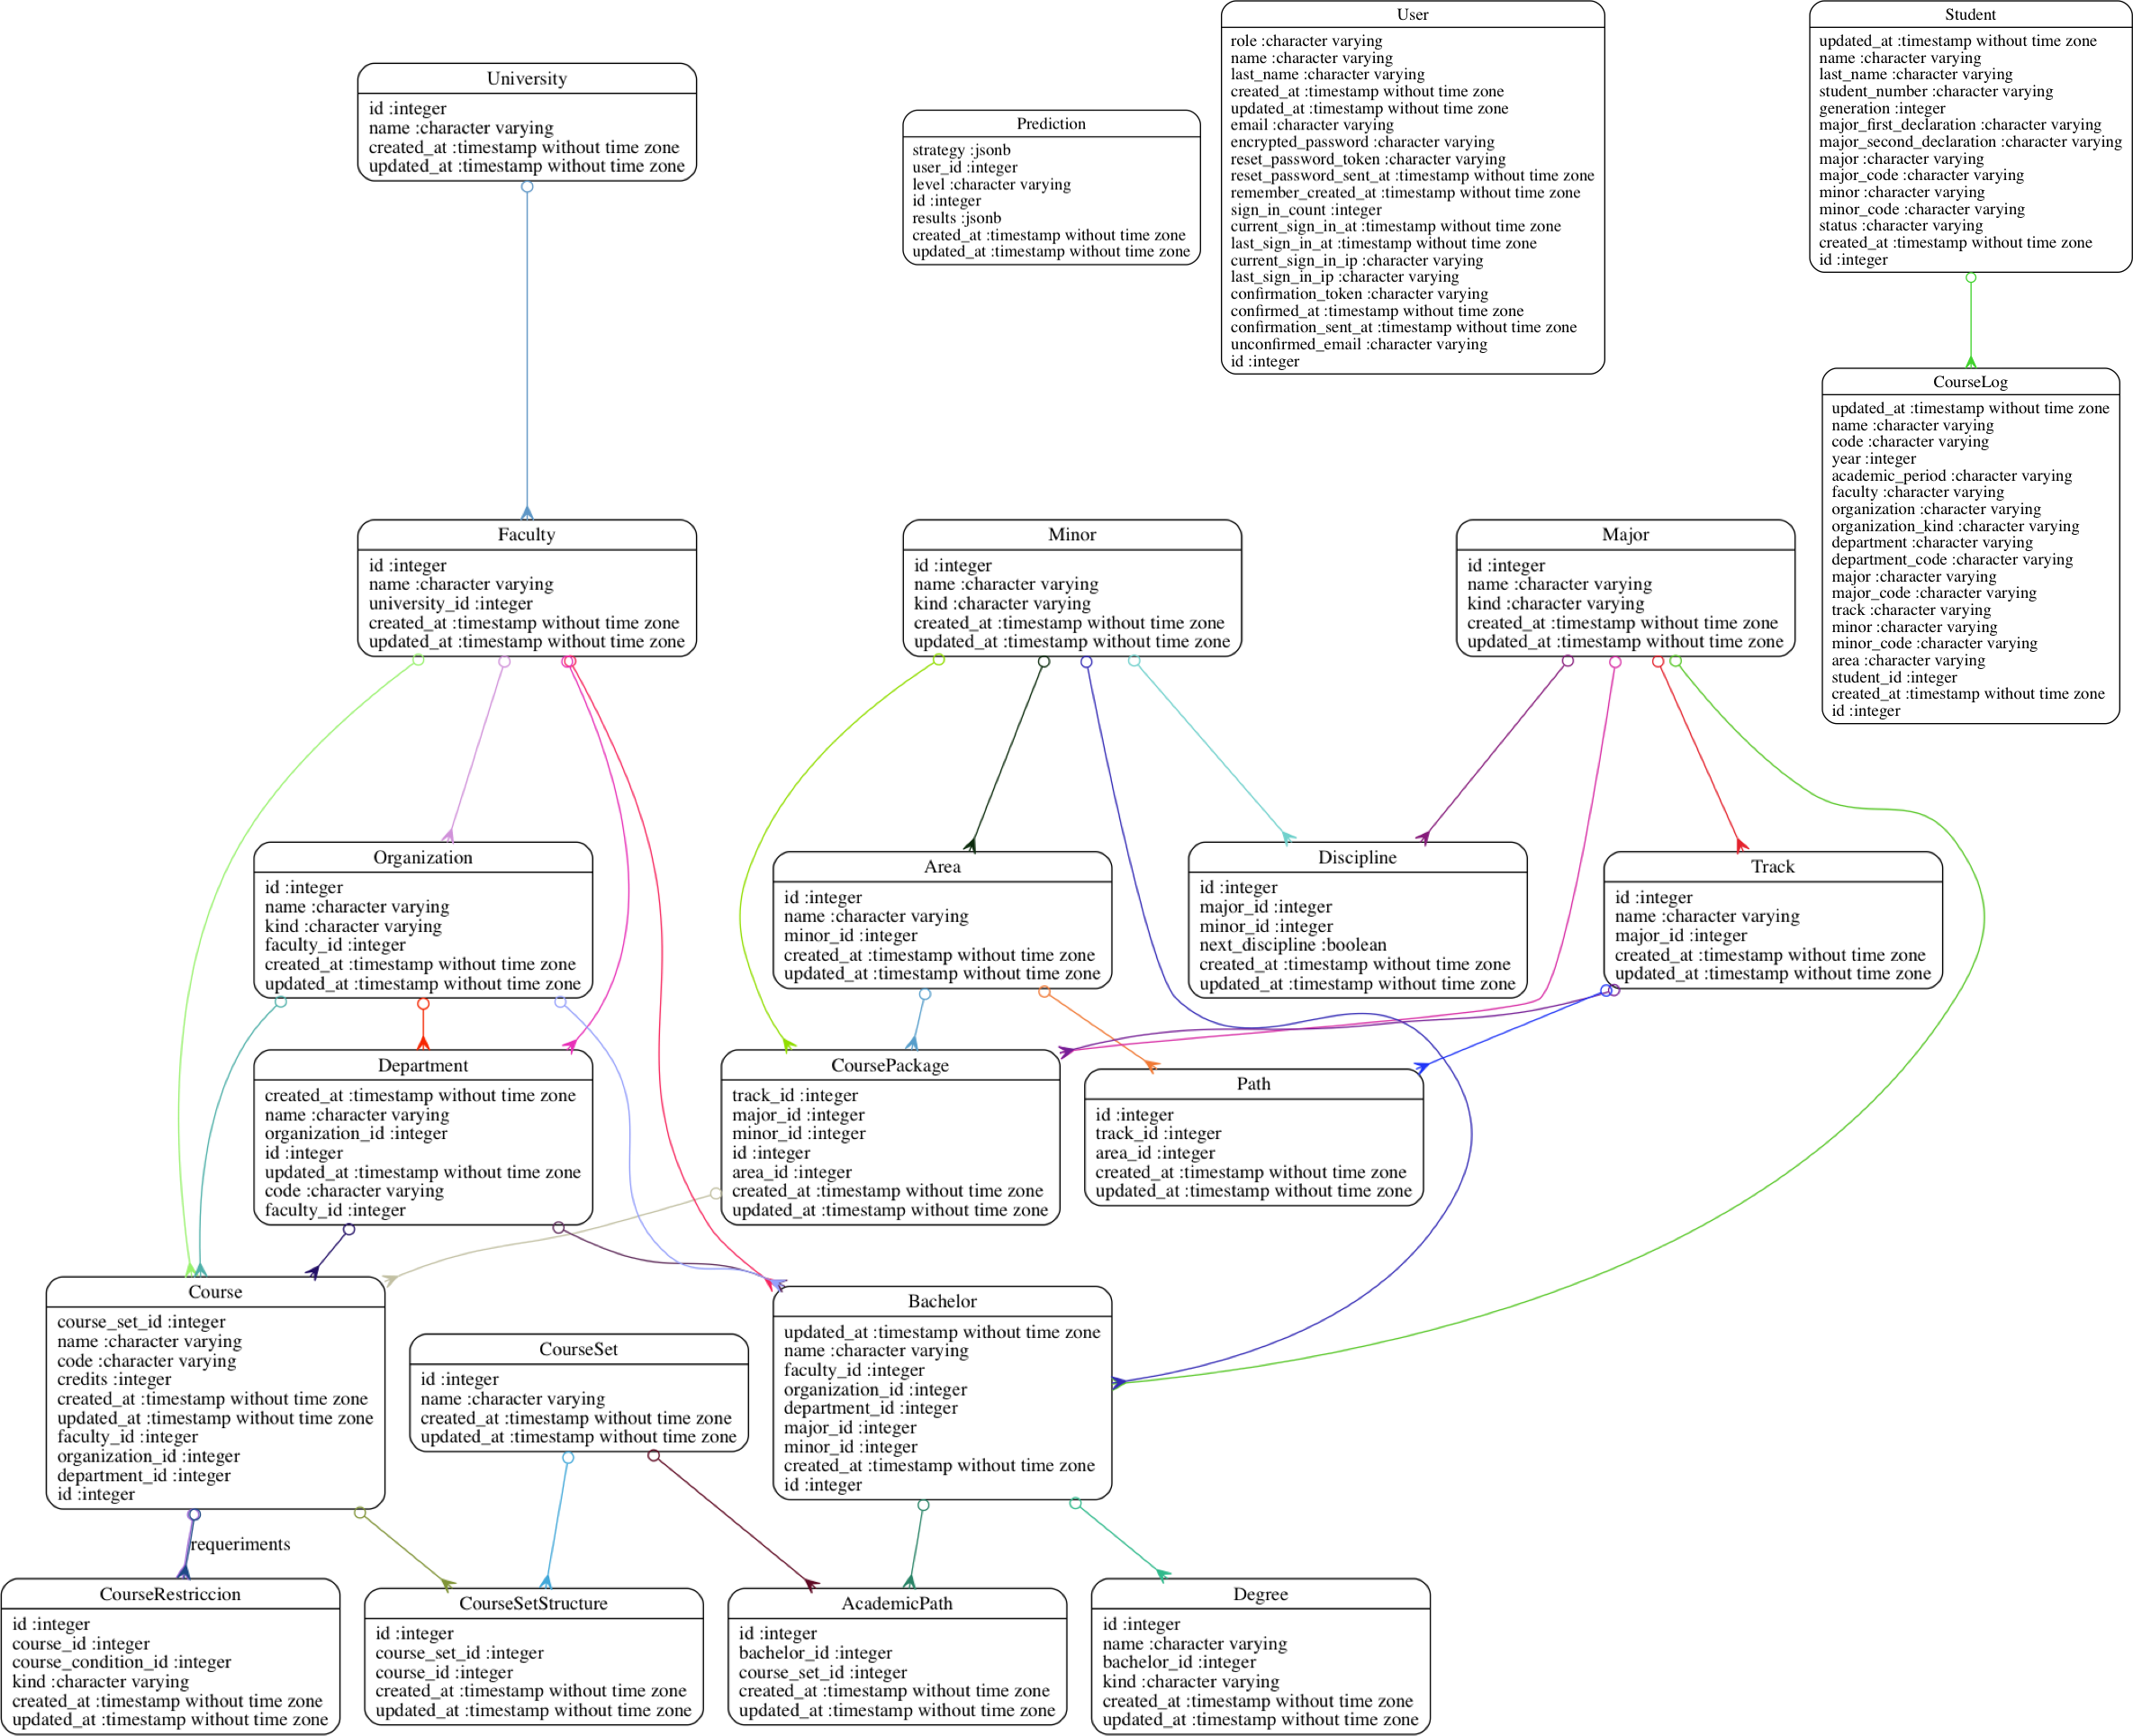
\includegraphics[width=0.95\textwidth]{./figures/chapter_03/04_modelo_de_datos.png}
			\setcaptioncitation{Fuente Propia}
			\caption{Modelo de Base de Datos}
			\label{fig:components_diagram_picture}
		\end{center}
	\end{figure}

Este modelo puede ser dividido de modo conceptual en las siguientes partes:

\begin{enumerate}
	\item \textbf{Universidad:} Las tablas \textit{University}, \textit{Faculty}, \textit{Organization}, \textit{Department}, \textit{Course} y CourseRestriccions permiten representar las relaciones entre la PUC, sus unidades académicas, los cursos que dictan y las requisitos que poseen.
	\item \textbf{Plan de Estudio:} El plan de estudio corresponde al conjunto de cursos que debe realizar un alumno para obtener un grado académico o título profesional UC. Las tablas que permiten almacenar esta información son: \textit{Bachelor}, \textit{Degree}, \textit{AcademicPath}, \textit{CourseSet}, \textit{CoureSetStructure}, \textit{Major}, \textit{Track}, \textit{Minor} y \textit{Area}. Además de las tablas intermedias descritas en el modelo de datos.
	\item \textbf{Predicciones de demanda:} Son las tablas que permiten llevar el registro de las predicciones solicitadas y sus resultados respectivamente. Las tablas que permiten esto son: \textit{Student}, \textit{CourseLog} y \textit{Predictions}. Cabe destacar que está última tabla posee un enfoque SQL y NoSQL debido a que posee dos columnas \textit{strategy} y \textit{results} en formato JSONB, el permite almacenar datos en formato JSON en representación binaria.
\end{enumerate}

El enfoque de diseño que se utilizó para el desarrollo de la base de datos fue modelo de Entidad Relación, para así permitir una mejor administración de unidades académicas, cursos y los alumnos dentro de la universidad en la plataforma. Con el fin de mantener las estadísticas y las predicciones de forma aislada , se crearon las tablas Student,CourseLog y Predictions.

\subsubsection{Carga Inicial \label{sec:initial_data_load}}

Dado que las proyecciones de demanda se basan en la información histórica del avance curricular de los alumnos se hace necesario poder cargar de forma inicial los elementos mencionados a continuación con el objetivo de poder realizar predicciones al momento de poner en marcha el sistema. Los elementos que cargan son los siguientes:

\begin{enumerate}
	\item \textbf{Universidad:} Nombre de universidad, facultades, centros de estudios (organization), escuelas (organization), departamentos, los cursos y sus requisitos o correquisitos de cursos.
	\item \textbf{Plan de Estudio:} Se hace la carga inicial de los major y sus tracks, minor y sus áreas, la relación entre ambos y los cursos pertenecientes a cada uno.
	\item \textbf{Avance Curricular:} Se hace carga del avance curricular de las generaciones del 2013 hacia adelante con la información actualizada hasta noviembre del 2016 entregada por Dirección de Pregrado.
\end{enumerate}

\subsubsection{Descripción de los Datos \label{sec:periodic_data_loads}}

Las cargas periódicas están enfocadas en mantener actualizada la información necesaria para las predicciones de demanda de cursos semestre a semestre, por lo tanto, se hace importante que el sistema cuenta con un sistema que permite realizar la carga de la siguiente información:

\begin{enumerate}
	\item \textbf{Información de Cursos:} Corresponde a la  carga masiva de cursos vigentes en la universidad, cabe destacar que el sistema no considera un curso en un periodo académico determinado, lo que busca es mantener actualizado sus cursos para determinar cuales son vigentes al momento de realizar una predicción.
	\item \textbf{Avance curricular de los alumnos:} Esta información es esencial para realizar predicciones más acertadas con el avance del tiempo.
\end{enumerate}

Ambas informaciones descritas anteriormente deben ser cargadas al finalizar un periodo académico, ya sea semestre o temporada académica de verano. El sistema posee un sistema de alerta que permite recordar a los usuarios administradores vía email y notificaciones en la plataforma web de que es necesario realizar este proceso. Debido a que cada año un semestre (primero o segundo) o temperada académica de verano inician y terminan en fechas diferentes, se crea una forma genérica para ir calculando un inicio y término ficticio, el cual es ajustable por un usuario administrador. Los criterios de cambio de periodo académico son los siguientes:

\begin{tabularx}{\linewidth}{@{}Y  Y  Y  Y@{}}
  \caption{Criterios de fechas para cambios de periodos académicos} \label{tab:university_structure}\\
  \toprule
  Periodo Académico	&	Fecha de Inicio Genérica	&	Fecha de Término Genérica
  \endhead
  \midrule
 	  Temporadad Académica de Verano (TAV) & 02 de Enero & 31 de Enero \\
  \midrule
  	Primer Semestre & 01 de Marzo & 15 de Julio \\
  \midrule
  	Segundo Semestre & 01 de Agosto & 15 de Diciembre \\
  \bottomrule
\end{tabularx}

Las fechas descritas anteriormente permiten al sistema cuán actualizada está su información con respecto al tiempo presente, se podrán efectuar predicciones siempre y cuando esta información esté actualizada al periodo académico anterior de cuando se desea realizar.


\chapter[CONCLUSIONS]{Conclusions}
\input{./chapters/conclusions.tex}

%%%%%%%%%%%%%
%       REFERENCES        %
%%%%%%%%%%%%%

\cleardoublepage
\phantomsection \label{references}
\bibliographystyle{apacite}
\renewcommand{\bibname}{REFERENCES}
\bibliography{Thesis}

%%%%%%%%%%%%
%      APPENDICES      %
%%%%%%%%%%%%

\appendix % It is like a chapter, so each appendix (A, B, C...) must to be considered as a section

\newpage
\section[Glosario]{Glosario} \label{dictionary}
\begin{enumerate}
  \item \label{refactoring} \textbf{\textit{Refactoring}}\mbox{}\\ Es el proceso de reconstrucción de código existente sin cambiar su comportamiento. Mejora los aspectos non funcionales del \textit{software}, por ejemplo, rendimiento.
  \item \label{tdd} \textbf{\textit{Test Driven Development}}\mbox{}\\ Proceso de desarrollo de software el cual se basa en la repetición de un ciclo de tres pasos. Primero, el desarrollador escribe un test automático que define el comportamiento deseado del software; segundo, se escribe la mínima cantida de código que hace el test pasar y ,finalmente, se hace un proceso de \textit{refactor} del código.
  \item \label{pair_programming} \textbf{Programación a pares}\mbox{}\\ Proceso de programación donde dos programadores participan en un esfuerzo combinado de desarrollo en un sitio de trabajo. Cada miembro realiza una acción que el otro no está haciendo actualmente: Mientras que uno codifica las pruebas de unidades el otro piensa en la clase que satisfará la prueba, por ejemplo.
  \item \label{continuous_integration} \textbf{Integración continua}\mbox{}\\ Práctica de desarrollo de software mediante la cual los desarrolladores combinan los cambios en el código en un repositorio central de forma periódica, tras lo cual se ejecutan versiones y pruebas automáticas. La integración continua se refiere en su mayoría a la fase de creación o integración del proceso de publicación de software y conlleva un componente de automatización (p. ej., CI o servicio de versiones) y un componente cultural (p. ej., aprender a integrar con frecuencia). Los objetivos clave de la integración continua consisten en encontrar y arreglar errores con mayor rapidez, mejorar la calidad del software y reducir el tiempo que se tarda en validar y publicar nuevas actualizaciones de software \cite{aws}.
  \item \label{focus_group} \textbf{Focus Group}\mbox{}\\ Tipo de técnica de estudio empleada en las ciencias sociales y en trabajos comerciales que permite conocer y estudiar las opiniones y actitudes de un público determinado \cite{abc}.
  \item \label{epic} \textbf{Epic}\mbox{}\\ Agrupación de relatos de usuarios. También son considerados relatos de usuarios más grandes \cite{epic}.
  \item \label{mvp} \textbf{Minimal Viable Product} \mbox{} \\ Producto con suficientes características para satisfacer a los clientes iniciales, y proporcionar retroalimentación para el desarrollo futuro \cite{mvp}.
  \item \label{ontoligical} \textbf{Ingeniería Ontológica} \mbox{} \\ es un campo de las ciencias de la computación y ciencias de la información que estudia los métodos y metodologías para construir esquemas conceptuales (ontología): ésta corresponde a la representación formal de un grupo de conceptos dentro de un dominio y de las relaciones entre esos conceptos. Una representación a gran escala de conceptos abstractos como acciones, tiempo, objetos físicos y creencias podría ser un ejemplo de ingeniería ontológica \cite{ontology_engineering}.
  \item \label{script} \textbf{Script} \mbox{} \\ Corresponde a una serie un conjunto de instrucciones programadas bajo un ambiente de programación único o mixto. Las instrucciones se escriben en función del lenguaje utilizado por el ambiente definido en el proyecto en el cual se utiliza.
\end{enumerate}


\newpage
\section[An Interesting Short Story]{An Interesting Short Story}
\input{./chapters/appendix2.tex}

\end{document}
